\def\year{2015}
%File: formatting-instruction.tex
\documentclass[]{IEEEtran}
%\documentclass[peerreview]{IEEEtran}
%\documentclass[onecolumn]{IEEEtran}
%\renewcommand{\baselinestretch}{2}
%\documentclass[letterpaper]{article}
%usepackage{aaai}
\usepackage{times}
%\usepackage{helvet}
%\usepackage{courier}
\usepackage{cite}
\usepackage{graphicx}
\usepackage{url}
\usepackage{amsfonts}
\usepackage{moreverb}
%\usepackage{mathtools}
%%
%\usepackage{float}
\usepackage{bm}
\usepackage{paralist}
%\usepackage{minted}
%%
% so we don't need to specify figures subdirectory in figure code
%\graphicspath{{./figures/}}
\usepackage{subfig}
%\usepackage{minipage}
%needed to change table colors
\usepackage[table]{xcolor}
%\renewcommand{\arraystretch}{1.75} % General space between rows (1 standard)
%\renewcommand{\baselinestretch}{2}
\renewcommand\IEEEkeywordsname{Index Terms}
%%
%\frenchspacing
%\setlength{\pdfpagewidth}{8.5in}
%\setlength{\pdfpageheight}{11in}
%\pdfinfo{
%\title (Activity Monitoring and Prediction for Humans and NAO Humanoid Robots using Wearable Sensors)
%Author (Saminda Abeyruwan, Faisal Sikder, Ubbo Visser, Dilip Sarkar)}
%\setcounter{secnumdepth}{0}  
%\title{Semi-Automatic Extraction of  Training Examples from Sensor Readings for Activity Monitoring and Prediction for Humans and NAO Humanoid Robots}
\title{Semi-Automatic Extraction of Training Examples from Sensor Readings for Tracking Human Activities}
%\title{Activity Monitoring and Prediction for Humans and NAO Humanoid Robots using 
%Wearable Sensors}
\author{{Saminda Abeyruwan}, {Dilip Sarkar}, {Faisal Sikder}, and {Ubbo Visser}
\thanks{ Authors are with
 the
Department of Computer Science, University of Miami,
  Coral Gables, FL, 33146, USA
{ emails:\{saminda, faisalsikder, visser, sarkar\}@cs.miami.edu};
\today} }
 \begin{document}
 %\begin{sloppy}
% The file aaai.sty is the style file for AAAI Press 
% proceedings, working notes, and technical reports.
\maketitle
\IEEEpeerreviewmaketitle

\begin{abstract}
While humans perform activities of daily life, an accident 
such as a fall may occur. This might cause injuries to the human body, and immediate identification of it can alert for a fast response.  Currently, a plethora of inexpensive wireless motion sensing devices are available or can be assembled using off-the-shelf components. They are being used to collect motion data to monitor non-fall activities and fall events. However, there are remaining problems such as automatic extraction of motion features that distinguishes among the prior categories. We have developed a framework to setup a wireless sensor network collecting motion data. We also have introduced a novel method for semi-automatically extracting training examples from the motion data. We have developed a two-level classification network to accurately identify each type of non-fall activities and fall events. The proposed classification-network is a combination of neural and softmax regression networks.  Our empirical evaluations of the proposed two-layer network show that seven types of non-fall activities and four types of fall events are classified on our datasets with 100\% accuracy. 
\end{abstract}

\begin{IEEEkeywords} Fall detection, learning algorithms, neural networks, {MEMS}, 9-axis sensor, semi-automatic extraction of training examples, softmax.
\end{IEEEkeywords}

%\tableofcontents

\section{Introduction}
\label{sec:Intro}
%Justification for activity monitoring
Fall is a major cause of injury to the elderly population \cite{Rubenstein2006}. 
Each year about 30-60\% of the elderly population have one or more falls, and  about 10-20\% of these falls results in injury \cite{Rubenstein2006}. 
As reported in the Centers for Disease Control and Prevention (CDC) website 
\cite{CDC2014July},
``In 2010, falls among older adults cost the U.S. health care system \$30 billion in direct medical costs, when adjusted for inflation.'' By 2020 it is expected to reach \$67.7 billion. 
\par 
The availability of inexpensive miniature \emph{microelectromechanical system} (MEMS) sensors  has motivated researchers  to study their potential for assessing fall-risk  (see \cite{shanyReview2012}, \cite{howcroftReview2013}, and the references therein) as well as monitoring \emph{activities of daily livings} (ADLs) \cite{alvarezActivityAndFallRecognotion2015,BaoActivityrecognition2004,DernbachActivityAndFallDetectionPhone2012,krishnanActivityRecognition2014,kumarActivitAndFallDetection2013} and \emph{fall events} (FEs) \cite{baekFallDetection2013,baiFallDetectionPhone2013,DernbachActivityAndFallDetectionPhone2012,dumitracheFallDetection2013,kumarActivitAndFallDetection2013,leoneFallDetection2013,liangFallDetection2012,liFallDetection2009,moyaFallAndDamageDetection2015,ojetolaFallDetection2011,ShenFallDetectionPhone2015,steidlFallDetection2012,DoukasFallDetection2011,ErdoganFallDetection2014,JianFallDetection2015}. These studies have used  accelerometers,  or gyroscopes, or magnetometers, or  a combination of them to collect motion datasets at  25 Hz to 200 Hz.  
\par
Earlier studies demonstrated feasibility of various miniature wired or wireless devices, and recent studies have focused on extracting knowledge from motion sensor data.  Results from past studies have proven  that hardware for MEMS sensor based \emph{intelligent} devices to \begin{inparaenum} [($i$)] \item assess fall-risks, \item monitor ADLs, and \item identify fall events have reached maturity and can be assembled from off-the-shelf hardware. \end{inparaenum}  

\par
Remaining major challenges include automatic development of \begin{inparaenum}[($i$)] \item firmware and software for collecting motion data and  extracting features specific to applications and users, and \item software module for making intelligent decisions utilizing features extracted from motion data. \end{inparaenum}
For example, a device with a 9-axis MEMS motion sensor to be used for identifying four fall events --- fall forward, fall backward, fall left, and fall right. The device must have firmware modules to collect motion data, to preprocess motion data, and to extract sufficient features from the preprocessed data for identification of all fall events. Also, the device must have a software module that takes the extracted features as input and  correctly recognizes which fall event has occurred.

%However, the challenges: How to gather \textbf{\emph{sufficient }} motion datasets and how to \emph{\textbf{automate }} extraction of required information form the datasets  for assessment of fall-risks.

%The humans as well as the biped humanoid robots performs similar activities --- such as, jogging, and running etc. While performing these routine 
%activities, accidents such as falls may occur causing damage to the human body or to the structural 
%components of the humanoid robot \cite{moyaFallAndDamageDetection2015}. 
%In the near future human-robot will cooperatively work together for solving problems that are difficult for both groups.  For instance, there has been an increasing demand in 
%domains such as rescue to use autonomous or teleoperated humanoid robots to complete high-risk 
%tasks, otherwise would have been lethal to a human subject. Therefore, we envision environments 
%where humans and humanoid robots collaboratively work to complete tasks. 
\par
Since both humans and biped humanoid robots have almost identical movements and are susceptible to 
similar accidents, we believe that the same devices are suitable for monitoring activities and fall events of both 
groups. Moreover, in the near future humans and robots will cooperatively work together solving problems that are impossible for either group but can be solved with  combined efforts of both groups.  For instance, there has been an increasing demand in 
domains such as rescue to use autonomous or teleoperated humanoid robots to complete high-risk 
tasks, that otherwise would have been lethal to a human subject. Therefore, we envision environments 
where humans and humanoid robots collaboratively work to complete tasks. 

\par
To validate our hypotheses, we developed a generalized approach for learning 
and predicting activities of both groups \cite{abeyruwanFlairs2015}.  We attached wearable sensing devices to collect
motion data and have used software tools to interpret the sensor data to distinguish 
between regular activities and fall events (see Fig.~\ref{fig:deviceWithSubjects}). 
<<<<<<< HEAD
In our study, fall and on-fall activities of biped robots were identified with 100\%  accuracy after using Kalman filter \cite{Welch:1995:IKF:897831} with appropriate thresholding, but same method would not be as successful for human subjects.  However, using Logistic Regression and \emph{Support Vector Machines} (SVM) true positive recognition for human subjects was as low as 90\%. The most \emph{ad hoc} and arduous part of our work was extraction of training datasets from the time series, which was part of the motivation for the work presented in this paper.
=======
In our study, fall and on-fall activities of biped robots were identified with 100\%  accuracy after using Kalman filter \cite{Welch:1995:IKF:897831} with appropriate thresholding, but the same method would not be as successful for human subjects.  However, using Logistic Regression and \emph{Support Vector Machines} (SVM) the true positive recognition for human subjects was as low as 90\%. The most \emph{ad hoc} and arduous part of our work was extraction of training datasets from the time series, which was part of the motivation for the work presented in this paper.
% to investigate the prospect of using external embedded 
%devices to identify activities on a NAO humanoid robot. 

%\par
%In this work, we concentrate on extracting training datasets and test datasets from time-series collected from the device. For each type of activity to be monitored we collect nine time-series using a 9-axis MEMS sensor.  
%
%Before we report our contributions, we provide a brief review of work related to identification of 
%human activity.  



%  The microcontrollers and embedded devices provide a flexible platform to build may 
% real world applications. In order to build these applications, a practitioner would require  
% flexible and reliable software solutions. A practitioner also may require to use more than one 
% functionality provided by the devices to build applications. Existing software solutions provide 
% facilities to build applications to a certain degree, but, they lack methods or systems to 
% integrate 
% multiple devices simultaneously without much user burden. We have developed  a state-of-the-art 
% open 
% source software solution to build heterogeneous applications on many devices, which can be 
% programmed on multiple operating systems. 
%%%% Commented below is the version in FLAIRS
%\begin{figure*}[!t]
%\centering
%\begin{minipage}{0.84\textwidth}
%\subfloat[]{\label{fig:fa}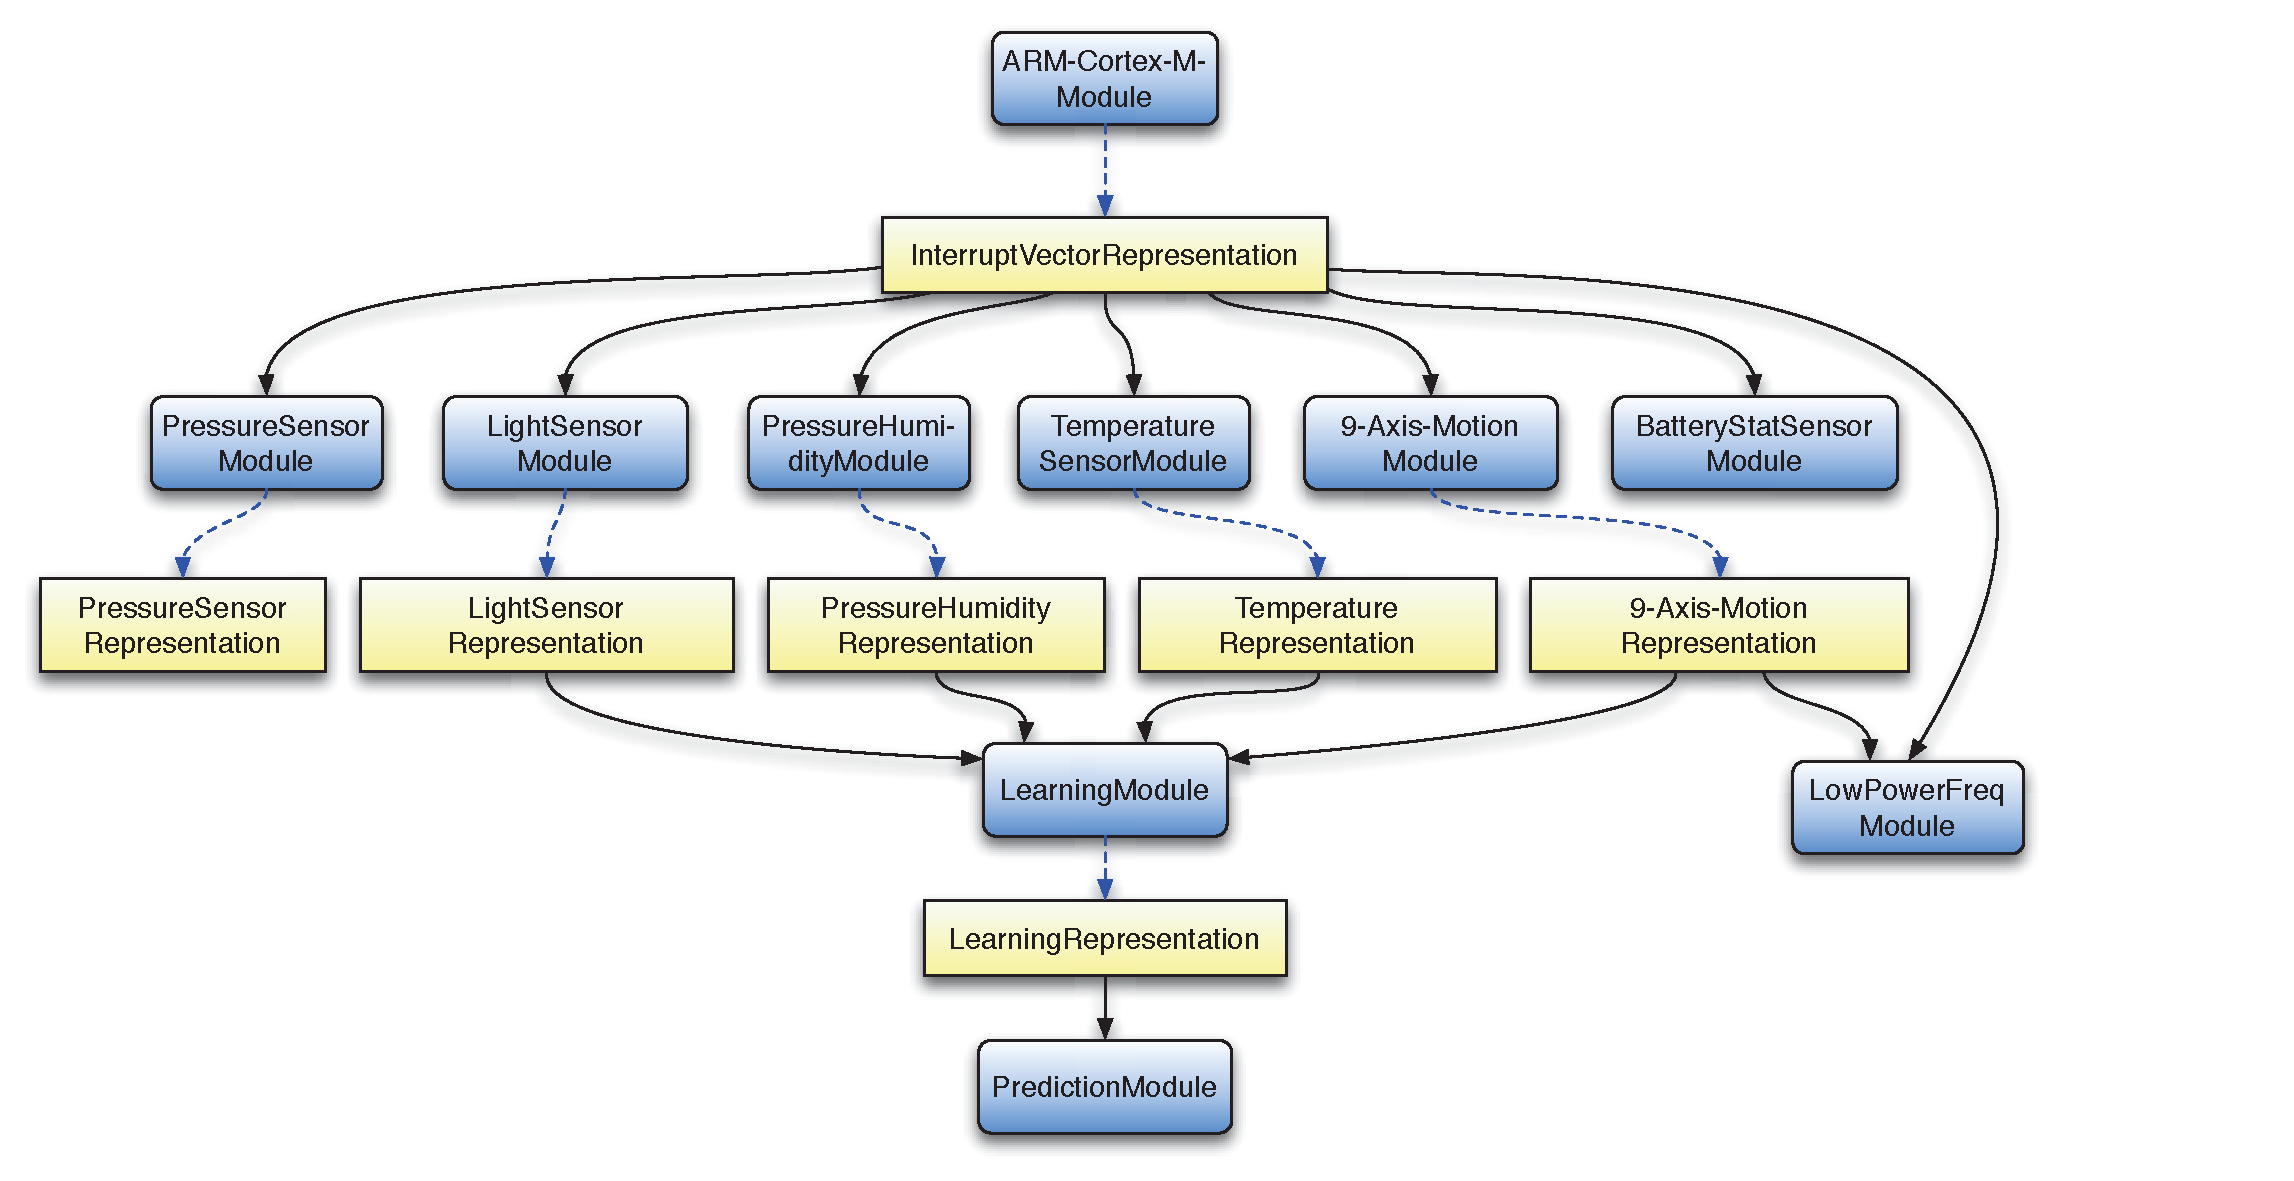
\includegraphics[width=\textwidth,height=3.5in]{figures/graph_structure_def-crop3.eps}}
%\end{minipage}
%\begin{minipage}{.12\textwidth}
%\begin{subfigure}
%\subfloat[]{\label{fig:fb}\includegraphics[width=\textwidth]{figures/human_figure.eps}}
%\end{subfigure}
%\begin{subfigure}
%\subfloat[]{\label{fig:fc}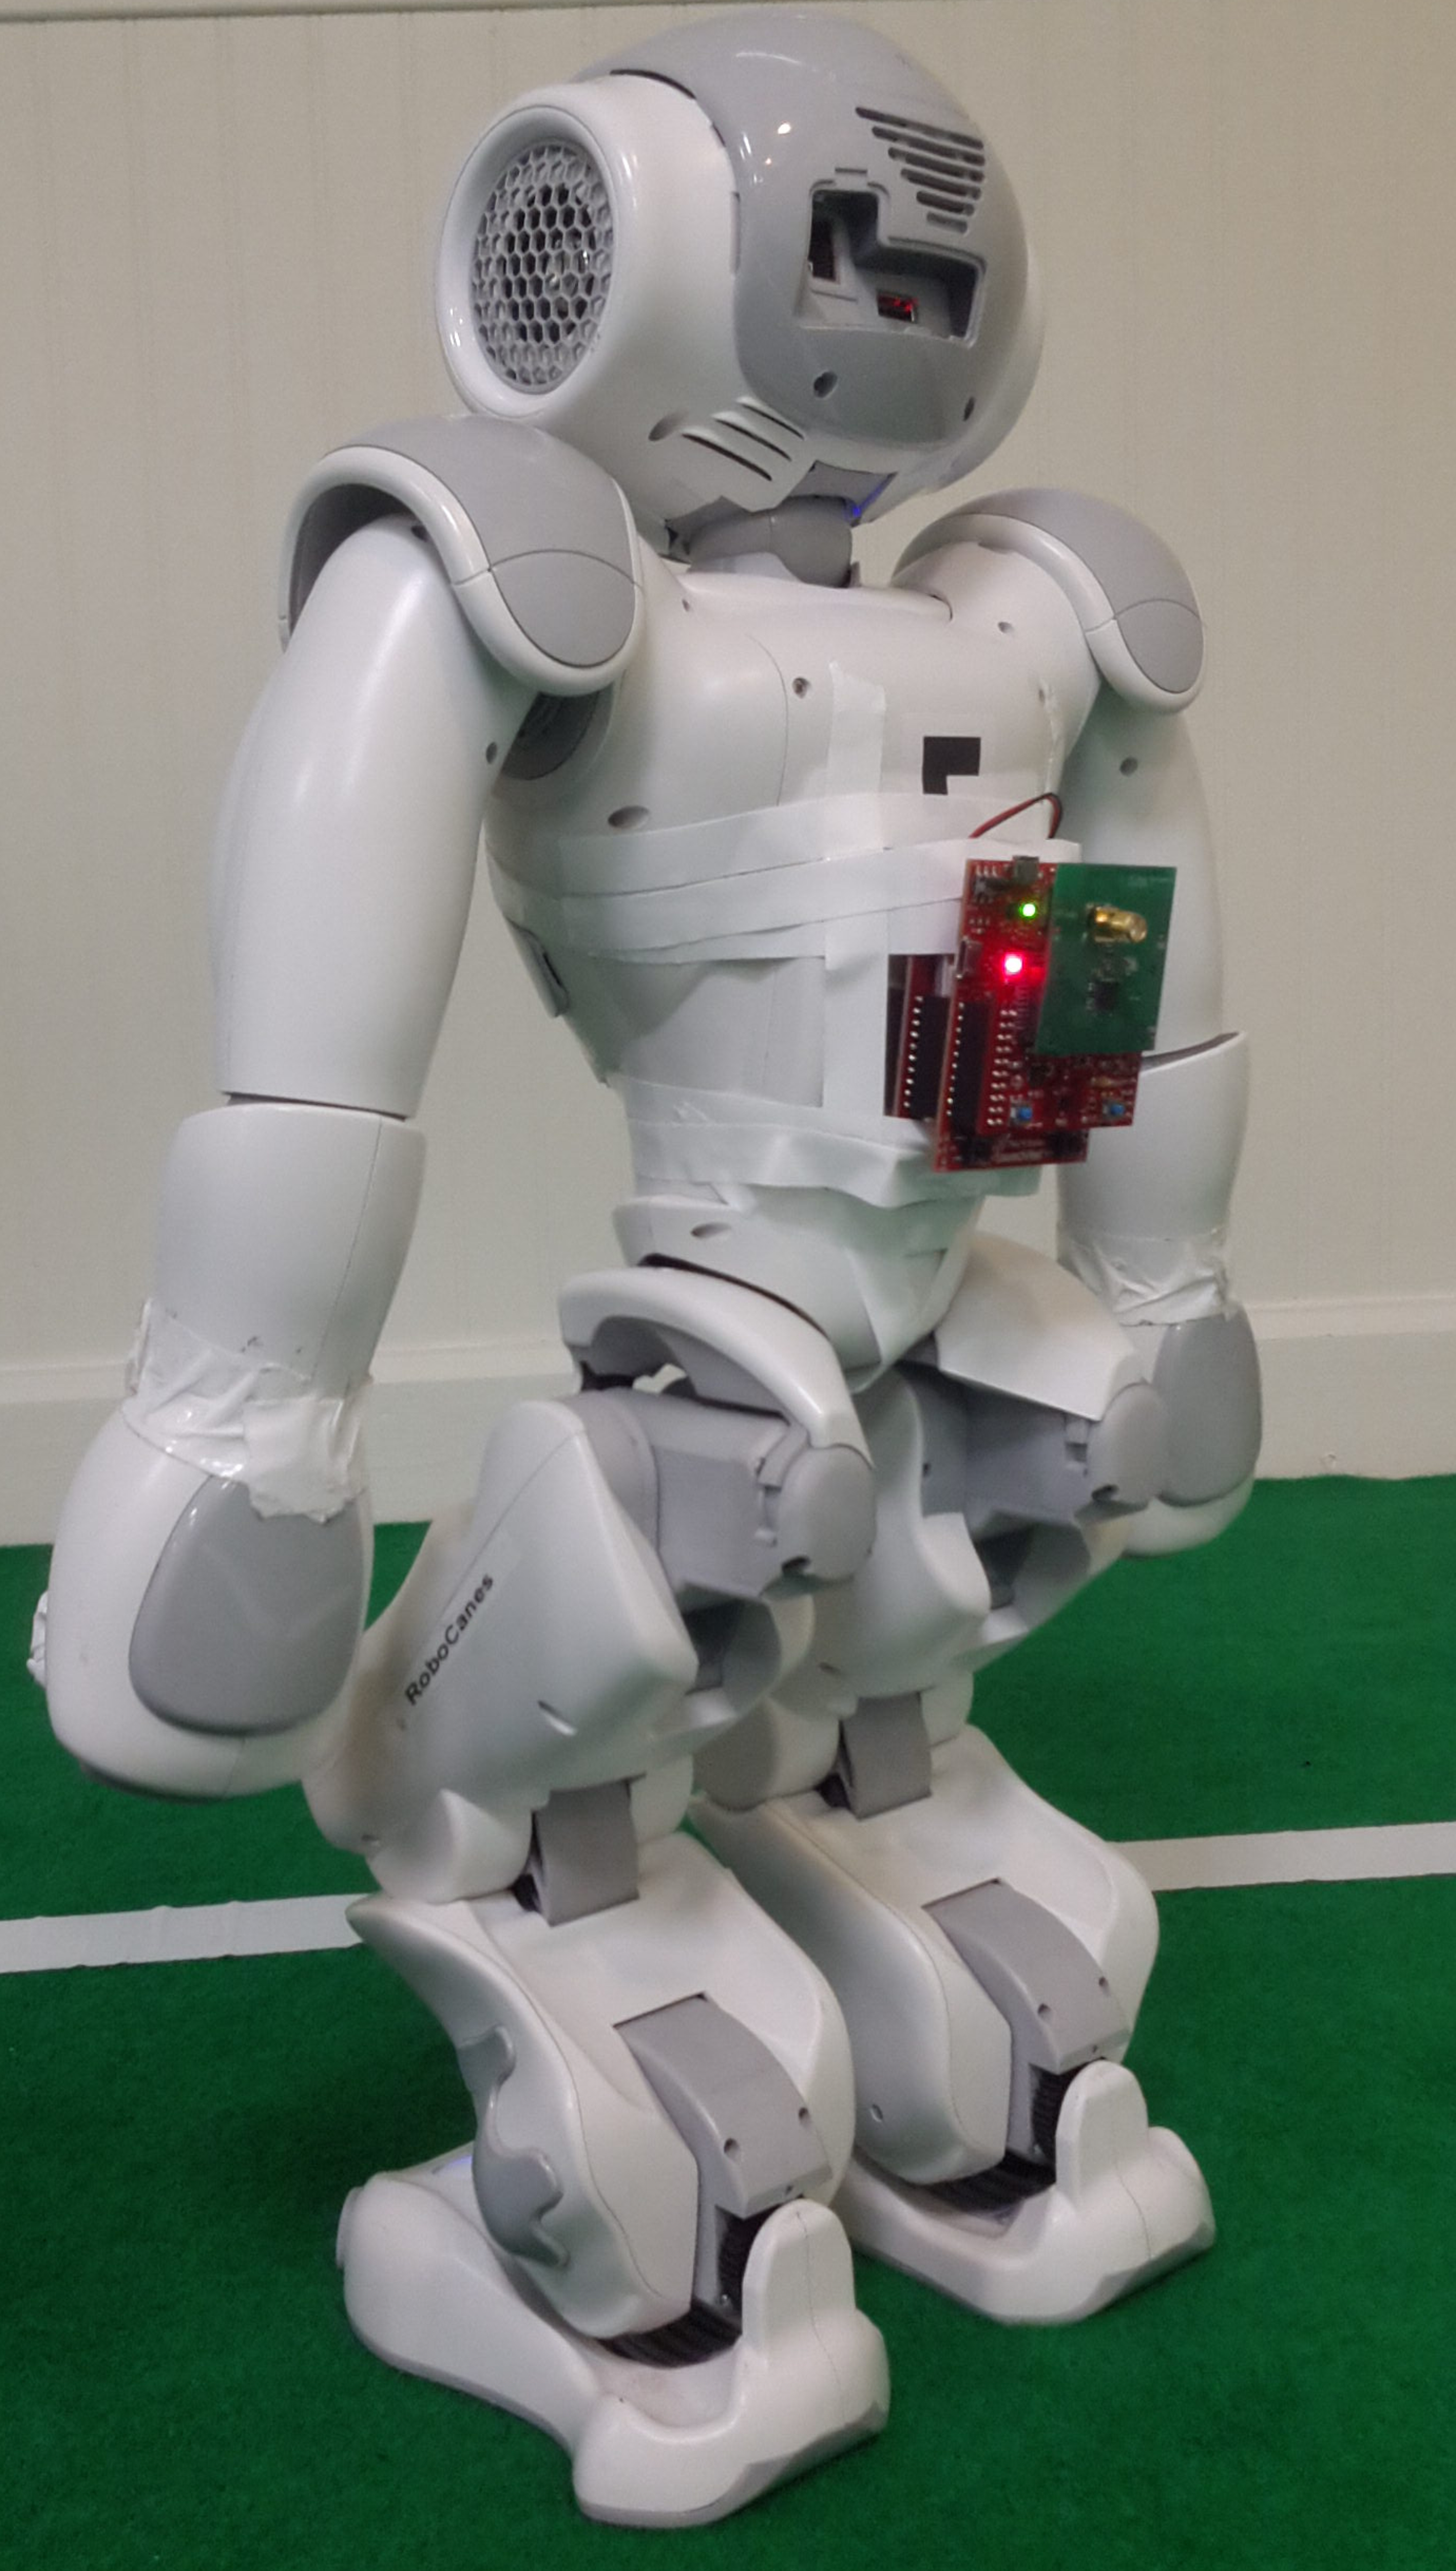
\includegraphics[width=\textwidth]{figures/robot_figure.eps}} 
%\end{subfigure}
%\end{minipage}



\begin{figure}[htb]
\centering
\subfloat[]{\label{fig:fb}\includegraphics[width=0.28\columnwidth]{figures/human_figure.eps}}
\qquad
\subfloat[]{\label{fig:fc}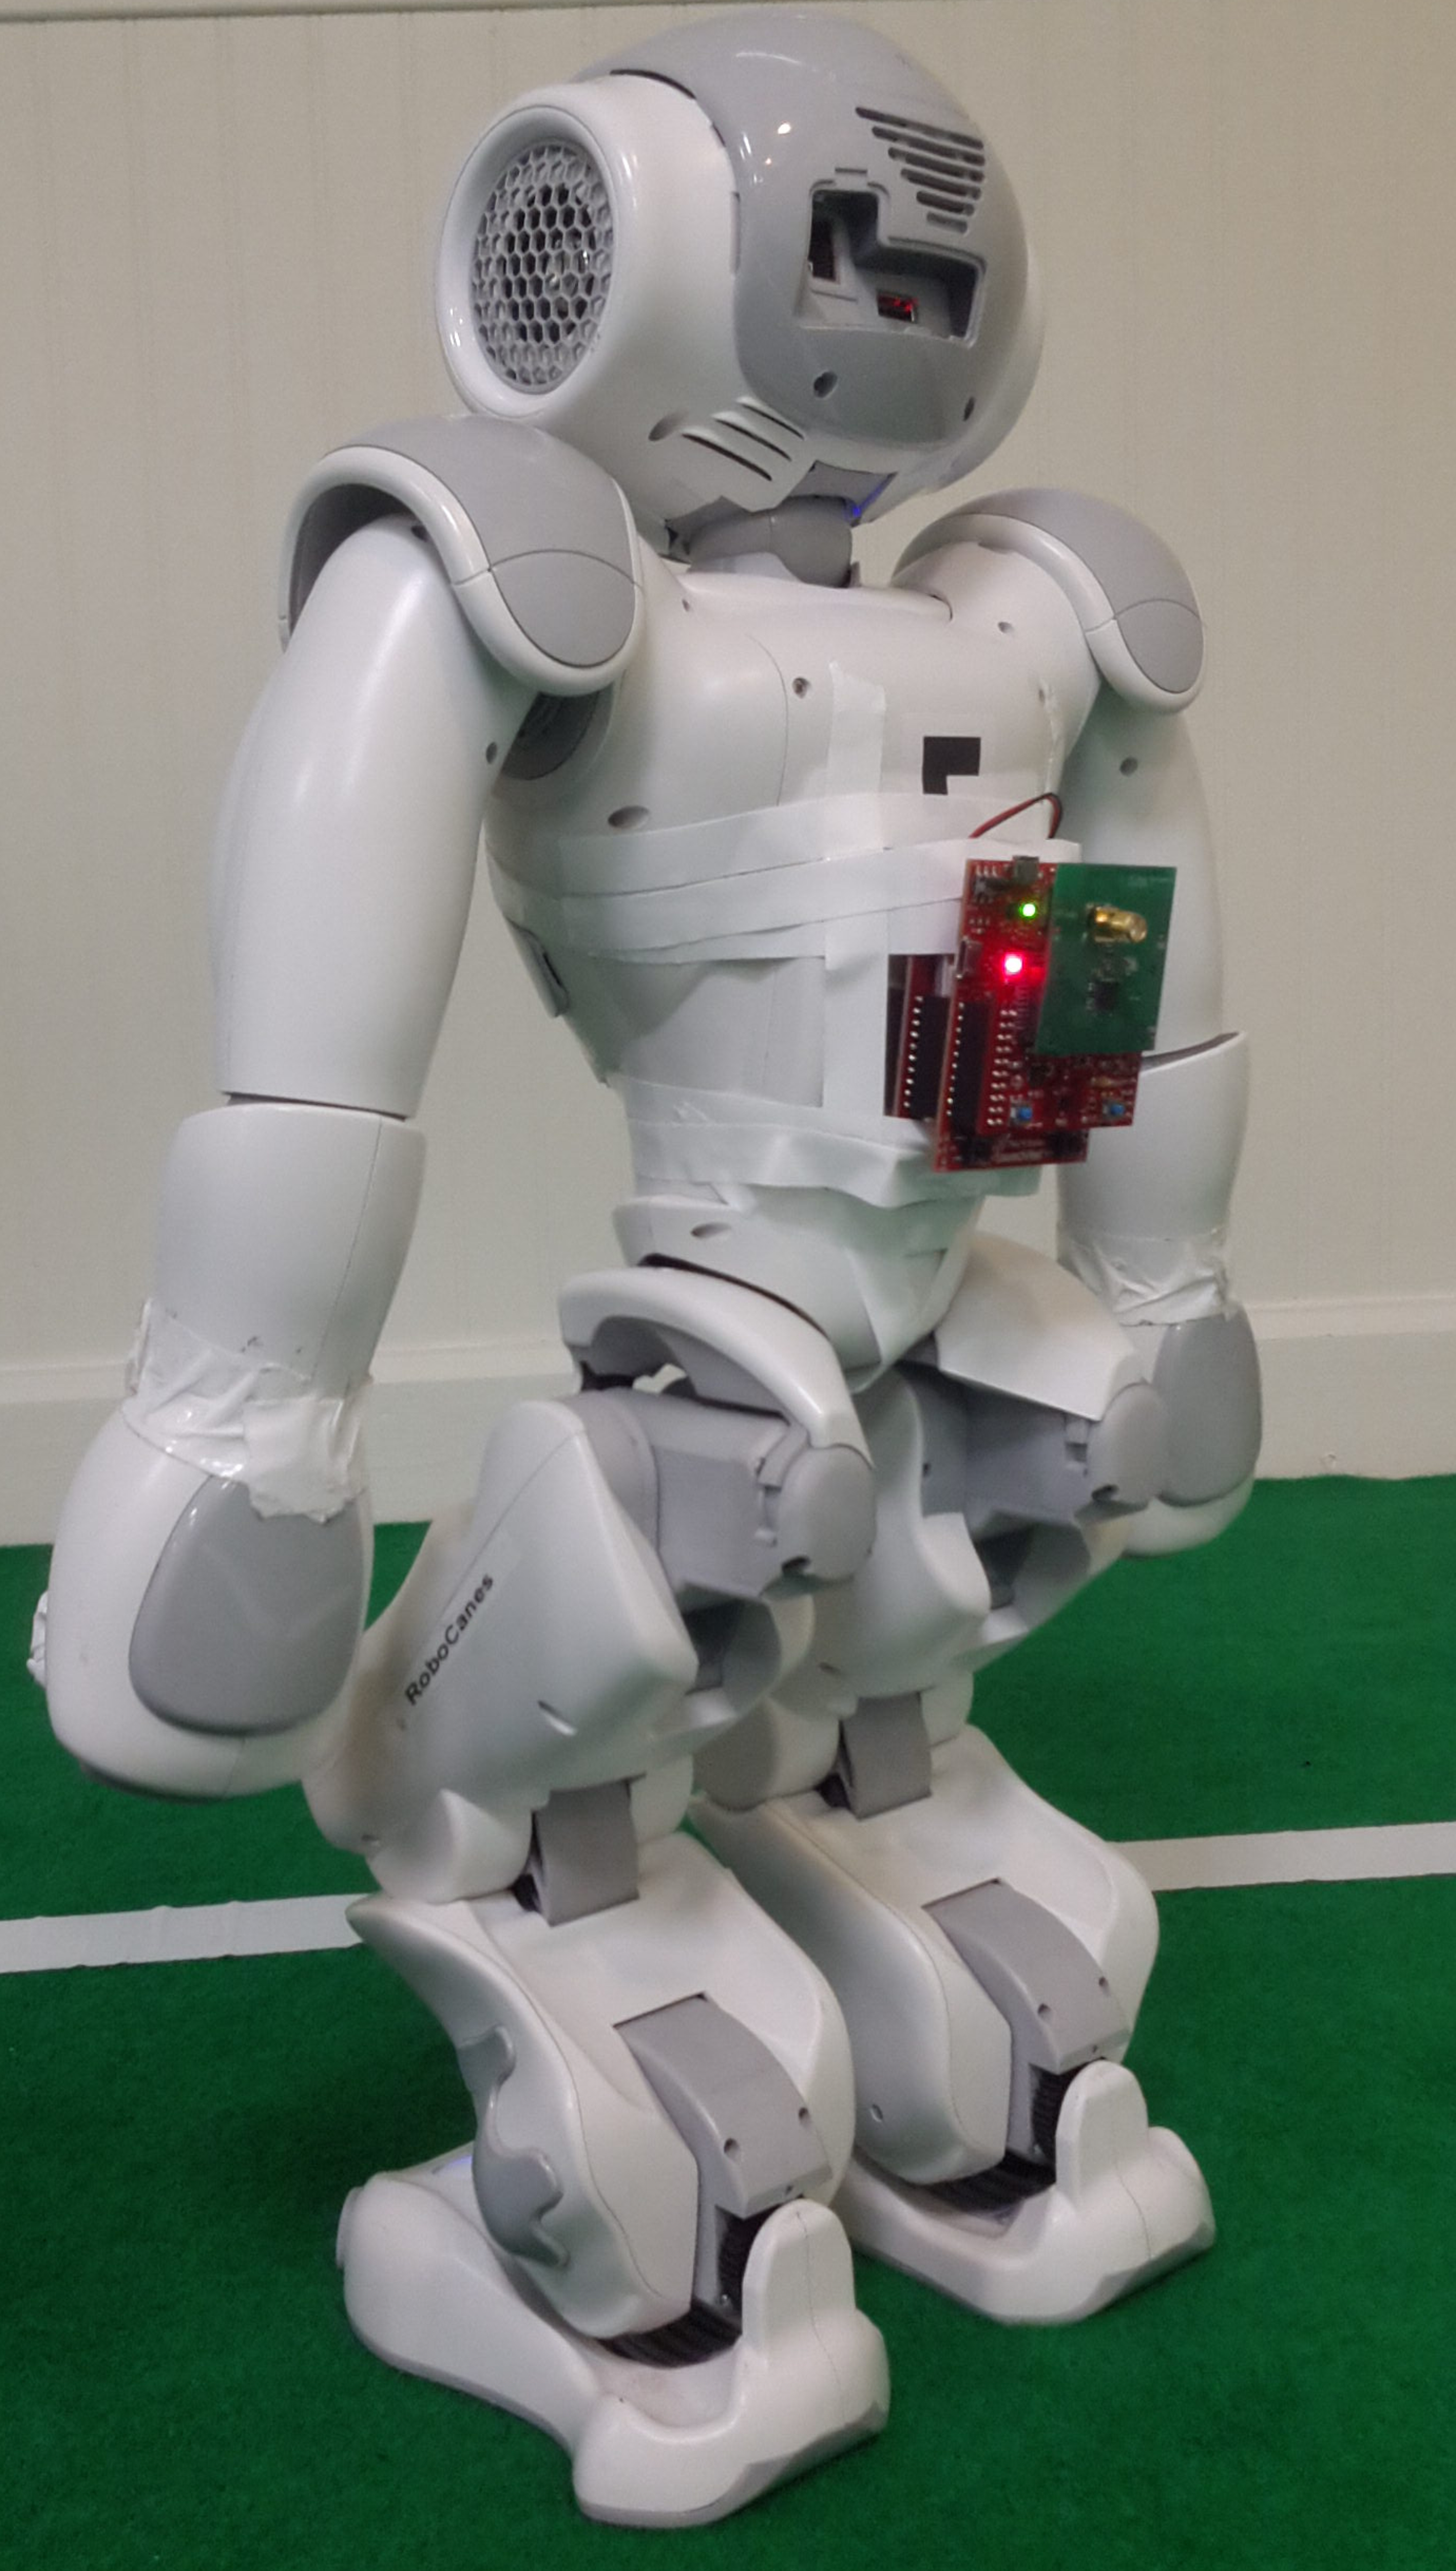
\includegraphics[width=0.25\columnwidth]{figures/robot_figure.eps}} 
\caption{(a) a wireless sensor device (assembled from a Tiva C Series  TM4C123G 
LaunchPad, a Sensor Hub BoosterPack, a CC2533 BoosterPack, and a Fuel Tank BoosterPack) 
attached to the back of a human subject; the device is running our framework  with only 
three motion-sensing modules; and (b) the 
same device configuration was used on the back of a NAO humanoid robot\cite{abeyruwanFlairs2015}.}
 \label{fig:deviceWithSubjects}
\end{figure}

\subsection{Our Approach and Contributions}

%Many off-the-shelf hardware boards, such as, TI microcontroller boards (MSP430{\texttrademark}LaunchPad, Tiva{\texttrademark} C Series 
%TM4C123G LaunchPad, Tiva C Series TM4C129 Connected LaunchPad) and add-on  BoosterPacks   with sensors as well as  wireless transmitter and receiver  provide flexible platform for 
%developing smart-devices for a wide rage of low power and portable applications. For our experiments, 
We have assembled a wireless sensing-device with a Tiva C Series TM4C123G microcontroller board, and three 
boosterpacks --- a
Sensor Hub BoosterPack  for sensing 9-axis motion,  a CC2533  BoosterPack for wireless 
networking, and a Fuel-Tank BoosterPack for power. We also assembled a wireless data collection device with a Tiva C Series TM4C123G microcontroller board, and a  CC2533  BoosterPack. These two devices were networked to create a wireless sensor network (WSN) for 
collecting motion data from  humans.
The data collection device is connected to a computer with a USB cable for logging sensed data.   

We have developed a set of software tools to create a framework that allow us
\begin{inparaenum}[($i$)] \item  to setup the WSN, \item to collect data, \item to extract training examples from sensor readings (see Section \ref{sec:SemiAutomaticExtractionOfTrainingVectors}), \item to learn from sample examples, and \item 
to monitor and predict events. \end{inparaenum} This framework is general enough for other practitioners to use the
available functionalities for creating WSNs, collecting data, learning, and prediction.

The rest of the paper is organized as follows: Related work is reviewed in Section~\ref{subSec:relatedWork}. In Section~\ref{sec:framework}, we describe the software development 
framework that we have proposed and implemented.
Section~\ref{sec:SemiAutomaticExtractionOfTrainingVectors} reports our novel methods for  
semi-automatic extraction  of \begin{inparaenum} [($i$)] \item training samples to be 
used by  learning algorithms  and \item testing data for activity monitoring. 
\end{inparaenum} Outlines of offline leaning algorithms used for teaching the device to 
identify activities and fall events are described in Section~\ref{sec:OffLineLearning}. 
 In the penultimate section, we present a detailed description of evaluation of proposed methods and also, report some typical results for humans.
%and NAO humanoid robots. 
%We have utilized two machine learning algorithms and a thresholding based method to learn 
%and identify normal and abnormal activities. Then we also have presented our observations and 
%discussion. 
Finally, the paper is concluded with a summary and future work.  

\section{Related Work}
\label{subSec:relatedWork}

Modern activity detection methods can be broadly categorized into two groups based on: 
\begin{inparaenum}[($i$)] \item inexpensive wearable embedded devices, and \item smart-phones. 
\end{inparaenum} Wearable embedded devices with add-on sensors provide options to develop effective 
activity recognition methods for humans and biped humanoid robots alike. The existing activity 
detection methods focus on special cases of fall detection both in humans and humanoid robots. These 
methods were primarily used in isolation.  Using readings from accelerometer and gyroscope a method for detecting four fall events --- forward, backward, right, and left - was reported in \cite{ojetolaFallDetection2011}.  The reported method utilized  a decision tree to 
learn and classify falls and activities of daily living (ADL). The method identified fall events 
with a precision of 81\%  and a recall of 92\%. 

Another detection method reported in\cite{baekFallDetection2013} used necklace-shaped tri-axial
accelerometer  and  gyroscope  sensors  for classifying  the  behavior  and  posture  of  human
 subjects. Their method distinguished between  ADLs and  falls, with  sensitivities  greater  than 
 80\%  and specificities  of  100\%. They experimented with ADLs such as: standing, sitting in the 
 chair or floor, laying, walking, running, going upstairs/downstairs, and bending, while, 
 falling forward, backward, leftward, rightward, and fall on the stairs were treated as abnormal 
 events. 
 
\cite{leoneFallDetection2013} prosed a system to detect events that cause trauma, and disabilities
using a tri-axial MEMS wearable wireless accelerometer. They used SVM or
classification of different events. \cite{BaoActivityrecognition2004} reported of using five 
small biaxial wire-free accelerometers attached  on the left bicep, right wrist, left quadriceps, 
right ankle, and right hip to recognize 20 activities starting from  walking  to  riding elevator  
to  strength  training to bicycling. They reported using decision table, instance-based learning, 
decision tree, and na\"{i}ve Bayes classifiers, where the decision tree variant showed the best performance 
with 84\% accuracy.  Similar efforts have been reported to detect human motions using motion 
tracking (see 
\cite{dumitracheFallDetection2013,kumarActivitAndFallDetection2013,krishnanActivityRecognition2014,gaoActivityRecognition2014,alvarezActivityAndFallRecognotion2015}).
 


{~\cite{moyaFallAndDamageDetection2015}} proposed a fall detection, avoidance, and damage 
reduction mechanism for biped humanoid robots. They tried to simulate the real world environment 
where humanoid robots have to walk over irregular surface, running or playing sports, collision 
with other robots. Their framework detected instability and performed fall avoidance or at 
least low-damage falling mechanism was invoked. Therefore, embedded devices  with add-on sensors 
provide a flexible platform to build may real world applications. 


There is an increasing popularity in using smart-phones to detect activities in health care domain. 
Using only the accelerometer readings from a smart-phone, \cite{baiFallDetectionPhone2013} analyzed five 
actions of human walking, running, standing up, sitting down, and jumping. They compared the 
acceleration characteristics of these actions with three different fall accelerations to infer the 
direction of the fall. Their method recognize the fall activity, only when a predefined set of 
conditions were met. But the method did not provide any prediction or indication value, that a fall 
may occur in future. 

\cite{steidlFallDetection2012} reported that the sensors of the smart-phones from different manufactures 
record values significantly incompatible ranges for identical tasks. Therefore, they trained a SVM 
classifier based on the features extracted from raw accelerometer readings and the directional 
changes of the constraining force exerted on an accelerometer to detect fall events. They compared 
these events to non-fall activities such as walking, running, jumping, and some actives which 
resembles falls such as sitting down on a chair. Their method detected fall events with 84.8\% average 
accuracy for different smart-phones. 

\cite{DernbachActivityAndFallDetectionPhone2012} explored methods to detect simple and complex activities using inertial 
sensors (accelerometer and gyroscope) of an Android smart-phone. The simple activities included: 
biking, climbing stairs, driving, running, sitting, standing, walking, and state of the phone not 
on the person. The complex activities were: cleaning, cooking, medication, sweeping, washing hands, 
and watering plants. Six different classifiers, multi-layer  perceptron (MLP), na\"{i}ve  Bayes,  
Bayesian  network,  decision  table,  best-first tree, and  K-star,  were trained on using the same 
feature extractor. For simple activities, 93\% accuracy using MLP were reported, while, 50\% 
success was achieved for complex activities.    

\cite{ShenFallDetectionPhone2015} used a  high-level fuzzy Petri net for the analysis and the development of 
identifying normal human actions such as sitting-down, squatting, walking, running, and jumping and 
abnormal events such as falling forward, backward, sideways, and vertical. Their fall detection 
method reported 94\% accuracy. One disadvantage of their process was that, some complex situations 
and movements cannot be detected accurately; e.g., falling down from  stairs, multiple collisions, 
or temporal unbalance motions.

\par 
To the 
best of our knowledge only three studies have been dedicated to biped robots \cite{Andre2015,Goswami2014,Moya2015}. The focus for these studies were prediction of a fall before it occurs and taking corrective measures to prevent the fall. The work reported in these papers are using readings from multiple sensors embedded in a robot for predicting a potential fall. On the other hand, our research goal is the proper identification of fall and non-fall events after they occur.


%Similar to existing methods, we have defined different normal and abnormal activities for humans 
%and NAO humanoid robots. In order to validate our hypotheses that the learning and predicting 
%methods unifies across the two groups, firstly, we have restricted the activities that can be 
%performed on a NAO robot. Therefore, in our experiments, the human performed activities that are 
%similar to the robot, such as, walk or falling forward/backward so forth. Secondly, we have 
%extended the human activities to more complex events.  We have used Texas Instruments 
%(TIs)  microcontrollers and boosterpacks for our experiments, 
%but, one can use microcontrollers and  sensor boards from other sources.  




\section{Framework for Data Collection and Processing}
\label{sec:framework}

A real-time or near real-time monitoring device performs a sequence of $n$ tasks $T = \{ T_1, T_2,\cdots,T_n\}$. A task $T_i$ may depend on another task $T_j$.  For satisfying dependence of a task on other tasks, it is necessary to create an \emph{execution order} on the set of tasks, if one exists. Denoting dependence of $T_i$ on $T_j$ as $D_{ij}$, a directed graph $G(T,D)$ can conveniently describe dependance among the tasks. A list of dependencies $D_{ij}$ completely describes the graph $G(T,D)$.
\par
We have created a generic framework for developing applications for \emph{data collection and processing}. This framework is described next.
%TODO: write an introduction paragraph for the section. For convince of reference for 
%Framework for Data Collection and Processing will be denoted by  FDCP. 

\begin{figure*}[!t]
\centering
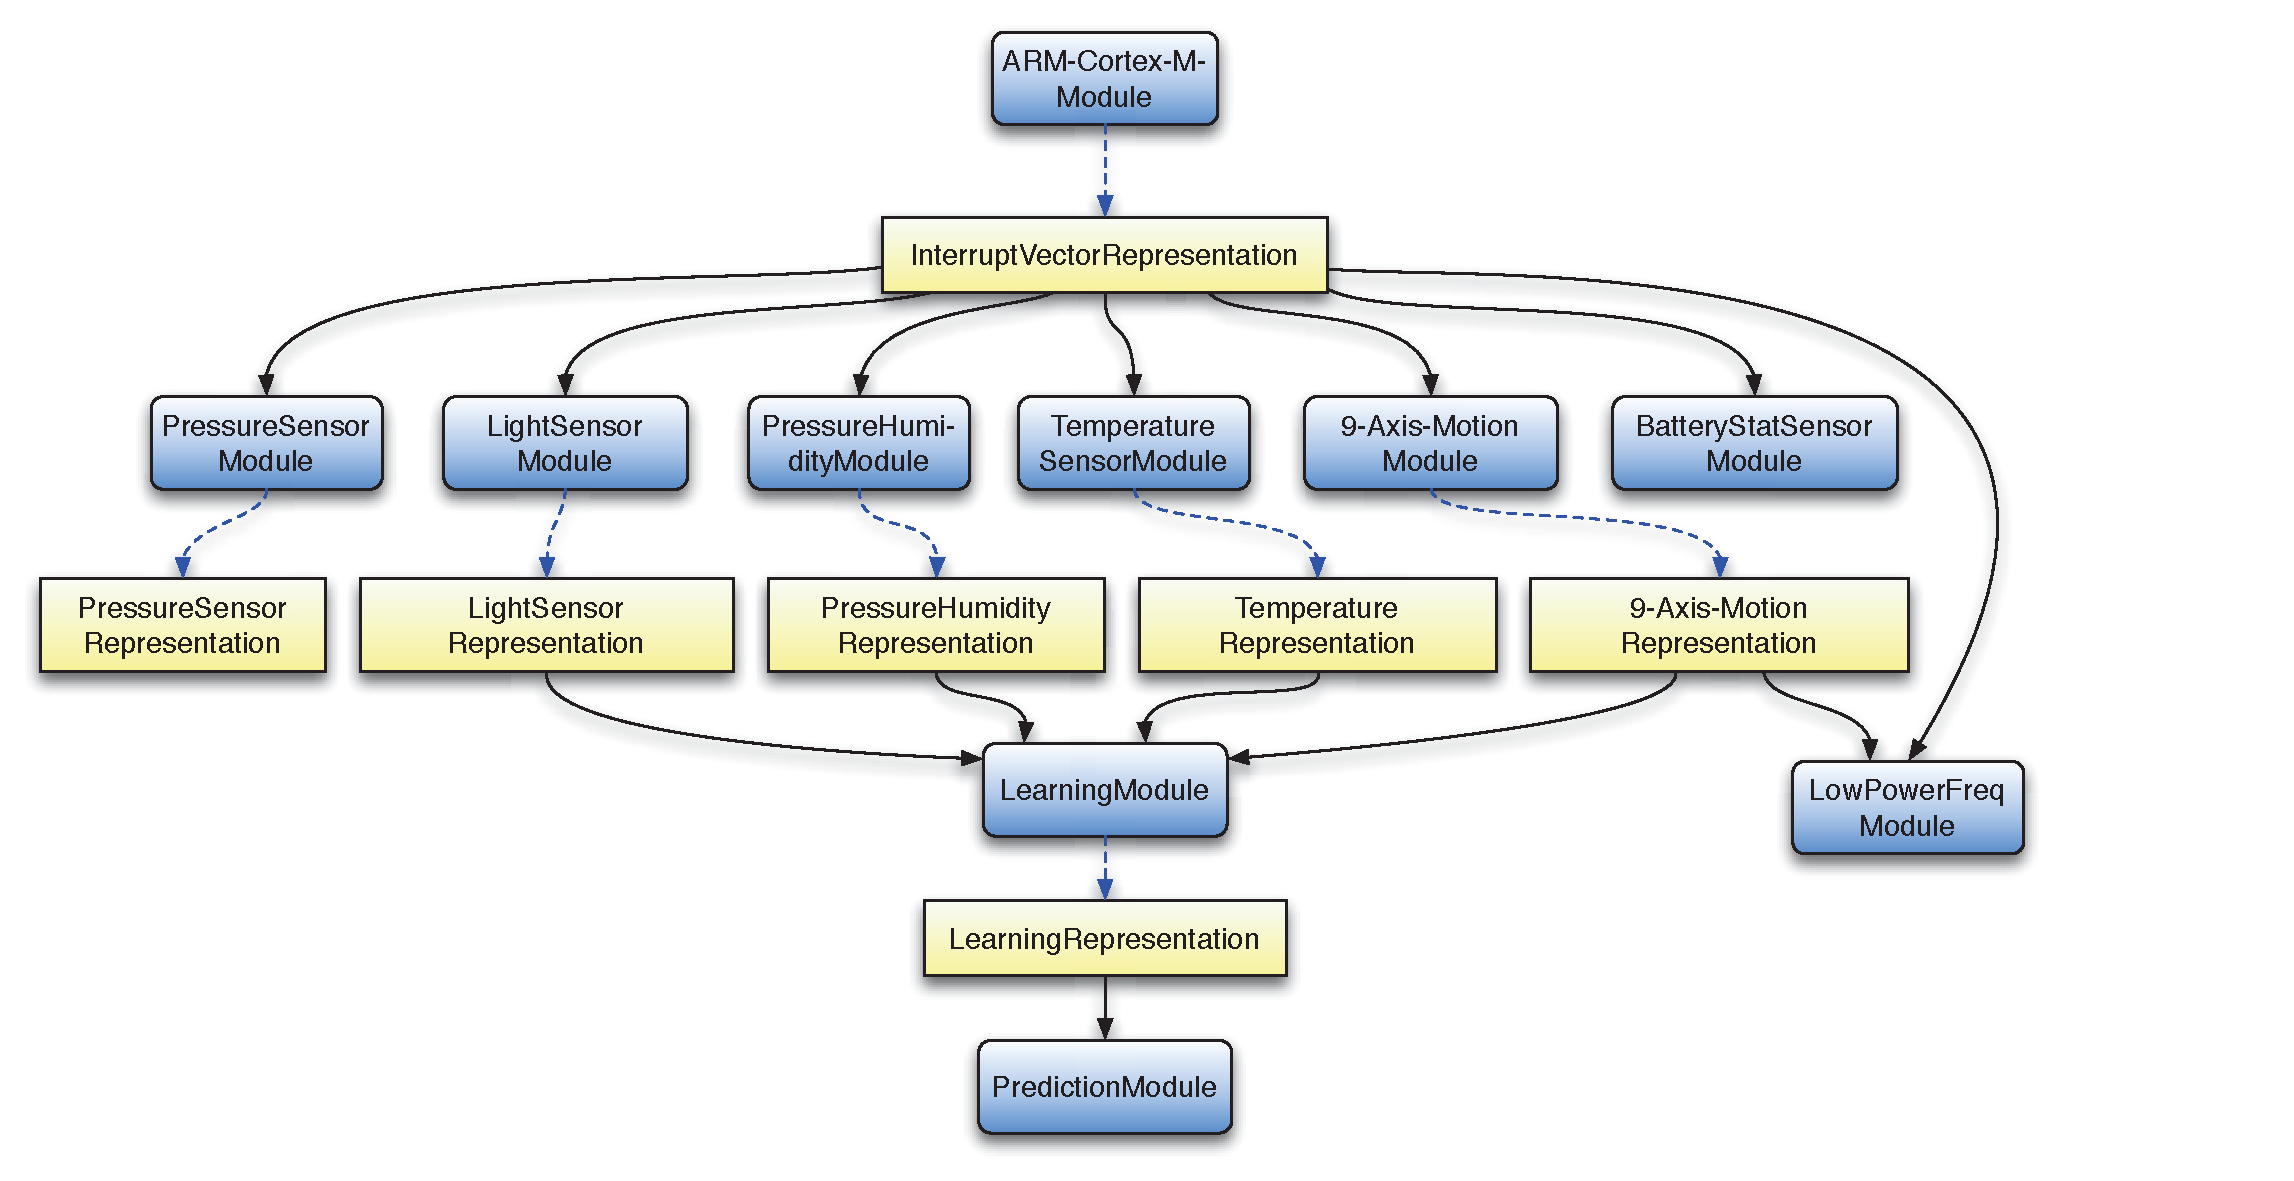
\includegraphics[width=.75\textwidth]{figures/graph_structure_def-crop3.eps}
\caption{Currently available software modules in our framework and a directed-graph representation of their functional relationship. Execution of a module (rounded-corner rectangle) generated data that is stored in the representation module (pointed-corner rectangle) for feeding into the next module.}
 \label{fig:framework}
\end{figure*}

\subsection{Overview of the Framework}
\label{sec:OverviewOfTheFramework}

\par
The framework provides generic functionalities to develop applications or rational agents 
on embedded devices that sense and actuate using add-on boards. The execution paths between sensors 
to actuators could contain complex behavior manipulations and modeling decisions that needs to be 
developed efficiently.
The framework 
includes: \begin{inparaenum}[($i$)] \item tools to develop modules and representations that execute on 
the microcontrollers or offline, \item the methods to access functionalities for physical 
robots, 
and \item a real-time visualization system\end{inparaenum}. Our framework is lightweight, flexible, 
and consumes minimum memory and computational resources. We have tested our framework on multiple 
microcontrollers and on boosterpacks. 
Our development framework, $\mu$Energia (\textit{pronounced as}: ``micro--Energia'') is available from the following web 
\textit{site}:
{http://muenergia.saminda.org}.

\subsection{Task-Schedule Generation Using our Framework}
\label{FrameWorkDescription}

%TODO: write what is meant by ``ordering''

We have divided each task into two components for an easier description and for the clarity of understanding: a {\em module} and one or more {\em representations}. A module implements executable code, while a representation exchange information from one module to another. Thus, a module may generate information for multiple representations as well as it may get inputs from multiple representations. 
\par
Once a user provides dependency descriptions, the framework converts it  into a directed graph (also know as precedence graph, or conflict graph).  If the graph has no cycle, the framework topologically sorts (see a book on algorithms such as\cite{Cormen:AlgorithmBook}), the nodes and creates an schedule for execution of the modules. In case the graph has one or more cycles, the framework reports so to the users.
For a visualization of the schedule, the framework  generates a directed graph. In this graph, modules are drawn as blue-shaded rectangles with rounded corners and the representations are drawn as yellow-shaded rectangles with pointed corners. The dependence of a modules on a representation is depicted as with a black arc with a solid line, while the dependency of a representation on a module is depicted with a blue arc with a dotted line. 
%We have tested our framework on multiple microcontrollers and on boosterpacks.

The directed graph in Fig.~\ref{fig:framework} shows a framework generated task-schedule 
for  a Tiva C Series TM4C123G microcontroller to collect and process data from 
\begin{inparaenum}[($i$)] \item Bosch Sensortec BMP180 pressure sensor, \item Intersil 
ISL29023 ambient and infrared light sensor, \item Sensirion SHT21 humidity and ambient 
temperature sensor,  \item  TMP006 non-contact infrared temperature sensor, and \item 
InvenSense 
MPU-9150 --- a 9-axis MEMS motion sensor. \end{inparaenum}

%\par
%The framework 
%includes: \begin{inparaenum}[($i$)] \item tools to develop modules and representations that execute on 
%the microcontrollers or off-line, \item the methods to access functionalities for physical robots, 
%and \item a real-time visualization system\end{inparaenum}. Our framework is lightweight, flexible, 
%and consumes minimum memory and computational resources. We have tested our framework on multiple 
%microcontrollers and on boosterpacks. 
%Our development framework, $\mu$Energia (\textit{pronounced as}: ``micro--Energia'') is availabe from
%\textit{site}:
%{http://muenergia.saminda.org}.


\subsection{An Application of the Framework}

%The Figure \ref{fig:fa} shows the modules and representations related to our 
%experiments, where the boxes represent the computational modules, while the rounded-boxes represent 
%the input to a module or an output from a module. For brevity, in the rest of the paper, the  
%{\em computational modules} are refereed as  {\em modules}. 
Our current project uses 
the module {\em 
9-Axis-Motion Module} that contains logic to read from or write to MPU-9150, a 9-Axis 
(Gyro+Accelerometer+Compass) MEMS MotionTracking device on the sensor hub booster pack. The {\em 
9-Axis-Motion Module} deposits data from the motion sensors to 
representation {\em 9-Axis-Motion Representation}, which are used by the {\em 
Learning Module}. The {\em LeaningModule} use the motion sensor data and creates {\em LearningRepresentation} for the {\em PredictionModule}. 

\par 

In the next section, we propose a method for the semi-automatic extraction of training examples from motion datasets. These examples are used to teach a device/system that identifies desired events. 

\section{Semi-Automatic Extraction of  Training Examples}
\label{sec:SemiAutomaticExtractionOfTrainingVectors}

This section and the next section provide our main contributions of the paper. Here, we provide a description 
of a method for semi-automatic extraction of training examples. This method has expedited our 
annotation 
of motion data considerably. As shown in Table~\ref{Tbl:ListOfActivities},  our study has considered four types of fall events: 
\begin{inparaenum}[1)] \item fall forward ({\sf FF}), \item fall backward ({\sf FB}), 
\item fall left ({\sf FL}), and fall right ({\sf FR}). \end{inparaenum} We have used the 
following seven activities:\begin{inparaenum}[1)] \item walk forward ({\sf WF}), \item 
walk backward ({\sf WB}), \item walk left ({\sf WL}), \item walk right ({\sf WR}), \item 
marching ({\sf MR}), \item rotate counter clockwise ({\sf RC}), and \item rotate 
clockwise ({\sf RA})  \end{inparaenum} as non-fall activities. 

\begin{table}[htb]
\caption{Activities and Fall Events and their abbreviations}
%\resizebox{\columnwidth}{!}
\centering
{
\begin{tabular}{|l|c|}
\hline
\textbf{Activity} & \textbf{Abbreviation} \\  \hline
Fall Forward &\textbf{FF} \\ \hline
Fall Backward &\textbf{FB}  \\ \hline
Fall Left &\textbf{FL}  \\ \hline
Fall Right &\textbf{FR}  \\ \hline \hline
Walk Forward &\textbf{WF} \\ \hline
Walk Backward &\textbf{WB} \\ \hline
Walk Left &\textbf{WL} \\ \hline
Walk Right &\textbf{WR}  \\ \hline
March &\textbf{MR}  \\ \hline
Rotate Clockwise &\textbf{RC} \\ \hline
Rotate Anticlockwise&\textbf{RA}  \\ \hline
\end{tabular}
}
\label{Tbl:ListOfActivities}
\end{table}

\subsection{Data Collection and Preprocessing  }
\label{subsec:preDataCollection}

We have setup the framework as described in Section \ref{sec:framework} and enabled the 
motion tracking device to sample at $20ms$, which is equivalent to 50$Hz$ 
sampling rate. The motion tracking device outputs nine values. Three-axis  
accelerometer readings are in  meter per square second ($m/s^2$), 3-axis gyroscope readings are 
in radian per square second ($rads/s^2$), and  3-axis magnetometer readings are  in 
Tesla ($T$). For experiments  and results reported here, we have excluded the magnetometer readings. Therefore, 
our input data vectors  are in $\mathbb{R}^6$ and they consist of accelerometer and 
gyroscope values. The plots of the raw motion datasets for fall forward and  walk forward 
events 
are shown in Figures~\ref{fig:human_fall_forward_crop} and 
\ref{fig:human_walk_forward-crop}, respectively. They demonstrate the complex nature of 
these time series, and indicate the difficulty of extracting features from them that are 
useful for training as well as monitoring of events and falls.

%\begin{figure}[htb]
%	\centering
%		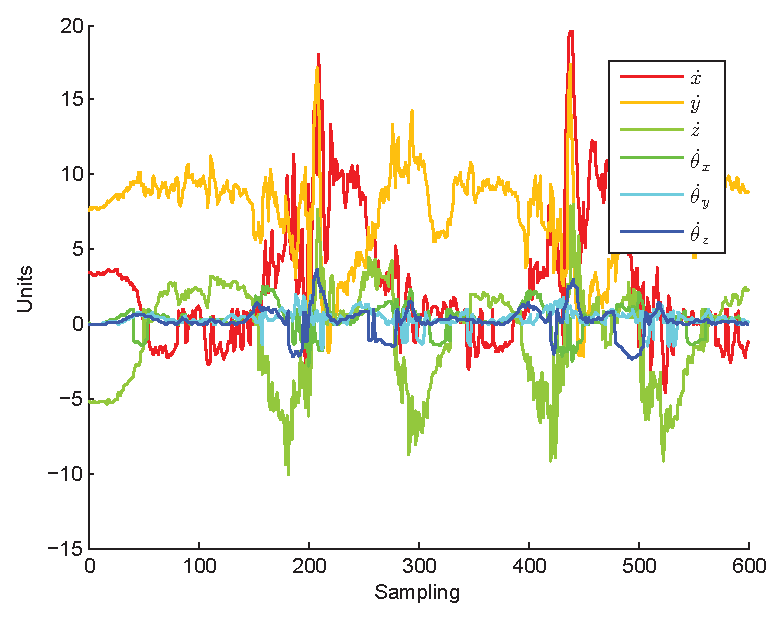
\includegraphics[width=0.95\columnwidth]{plots/human_falling-crop.eps}
%	\caption{Motion dataset for  Fall Forward event of a human subject}
%	\label{fig:human_fall_forward_crop}
%\end{figure}

\begin{figure}
\centering
  \mbox{\subfloat[Motion dataset for  fall forward event of a human 
  subject.]{\label{fig:human_fall_forward_crop} 
  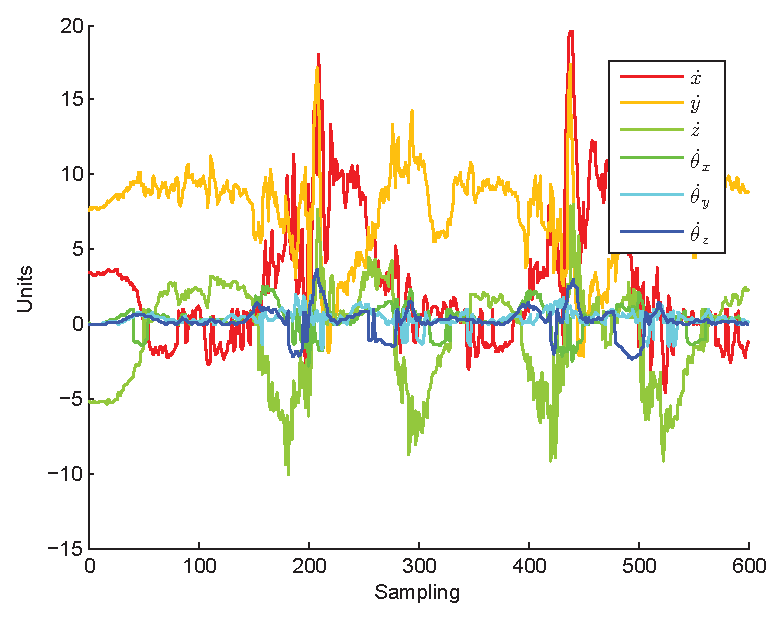
\includegraphics[width=0.9\columnwidth,height = 1.5in]{plots/human_falling-crop.eps}}}
  \mbox{\subfloat[Motion dataset for walk forward event of a human subject. 
  ]{\label{fig:human_walk_forward-crop} 
  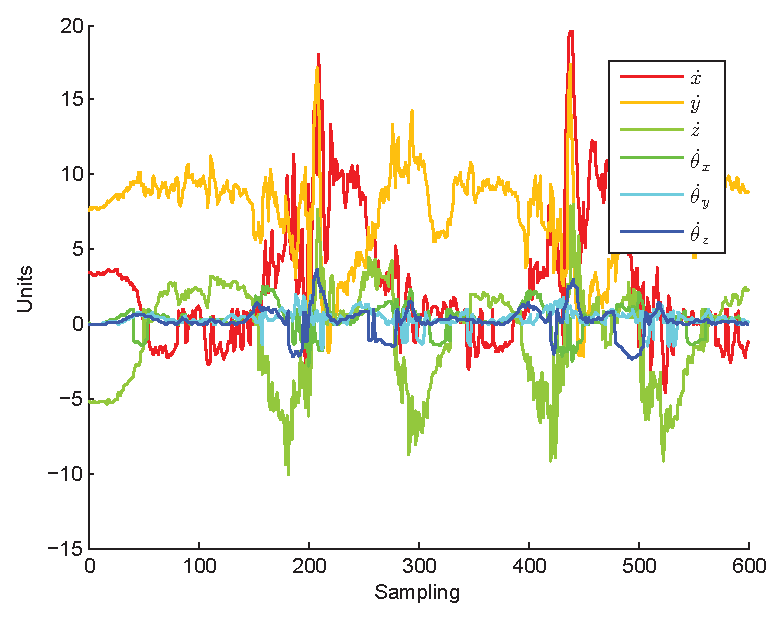
\includegraphics[width=0.9\columnwidth,height = 1.5in]{plots/human_falling-crop.eps}}}
  \caption{Fall and walk forward motion datasets. The accelerometer ($\dot{x}$, 
  $\dot{y}$, $\dot{z}$) and the gyroscope ($\dot{\theta_x}$, 
  $\dot{\theta_y}$, $\dot{\theta_z}$) readings are shown with the respective traces. }
\end{figure}


\subsubsection{Identify and Adjust for Missing Data Points}
\label{sec:IdentifyAndAdjustForMissingDataPoints}
Some data packets may be lost during transmission because of noise. We numbered each 
sensor reading sequentially and at the receiver the lost data points were identified from this number and was 
replaced using linear interpolation. Since only very few data points were lost and 
results obtained after linear interpolation was excellent, we did not experiment with other 
interpolation methods.

%\begin{figure}[htb]
%	\centering
%		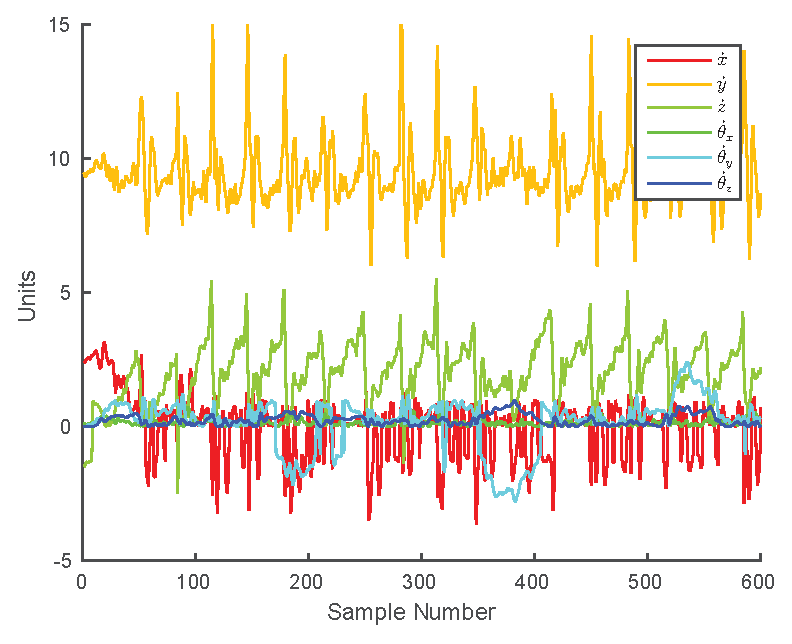
\includegraphics[width=0.95\columnwidth]{plots/human_walk-crop.eps}
%	\caption{Motion dataset for Walk Forward event of a human subject. }
%	\label{fig:human_walk_forward-crop}
%\end{figure}


\subsubsection{Noise Filtering}
\label{sec:NoiseFiltering}

After checking for missing data and adding interpolated values for the lost data,  high frequency noise was removed using a moving window averaging technique. We used a window  of 20 consecutive samples, which amounts to 400$ms$, 
and obtain the average value. Then the  window was moved by ten samples and average  value was computed again. The
process was repeated for each time-series of all motion datasets. Thus, we have allowed ten samples to overlap between windows. 
Selection of an overlap of ten samples is based on our empirical observation that a transition from non-fall event to a fall event takes about 500$ms$. Thus, averaged values will preserve transitions from non-fall events to fall events.   We have used the preprocessed time-series as the input to our automatic training example 
extraction method.


\subsection{Semi-Automatic  Extraction of Training Examples}

The barrier for collecting motion data is very low, if any. However, detection and identification of non-fall activities and fall events from motion data have remained an active area of research, as can be seen from the large number of recent publications. One of the main unsettled issues is how to characterize features from motion data that can be extracted easily for training and monitoring. In this section, we describe a method that semi-automatically extracts feature vectors that characterize non-fall activities and fall events.

The flow chart of the method used for extracting training examples are shown in Fig.~\ref{fig:FlowChartforAlgorTrainingExamples}. All the collected datasets were annotated as described next. If a dataset was for simulated-fall events, the dataset was treated as a 6-dimension vectors for clustering them into two clusters. We explored K-Mean and Gaussian Mixture clustering techniques. For completeness a brief description of each is provided next.

%TODO: first paragraph => why we need SATEE. Because of the difficulty of generating 
%training data. Then, description of the algorithm, with the figure (training data only). 
\begin{figure}[htb]
	\centering
		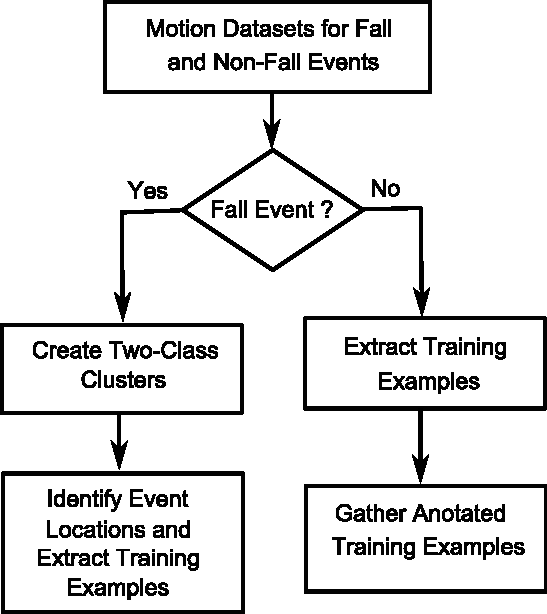
\includegraphics[width = 0.65\columnwidth]{figures/FlowChartAlgoForTrainingExamples.pdf}
	\caption{Flow chart of an algorithm for semi-automatic extraction of training 
	examples}
	\label{fig:FlowChartforAlgorTrainingExamples}
\end{figure}

\subsubsection{K-Mean Clustering\cite{Bishop:2006:PRM:1162264}}
K-mean clustering aims to partition a set of $n$ observations into $k$ clusters. Each 
observation is assigned to the cluster with the nearest mean. Let 
\{($\mathbf{x}^{(i)}$)\}$_{i=1}^n$  be the set of $n$ 
observations, where each observation $\mathbf{x}^{(i)}$ is a $d$-dimensional real vector 
and is 
assigned to one of the $k$ sets $\mathrm{S}_j \in \mathcal{S}$, for $ 1 \leq  j \leq k$ so 
that 
within-cluster 
sum of squares is minimized. Formally,

$$ \min _{\mathcal{S}} \sum_{i=1}^{k} \sum_{\mathbf{x} \in \mathrm{S}_i} || \mathbf{x} - 
\boldsymbol{\mu}_i 
||^2,$$
where $\boldsymbol{\mu}_i $ is the mean of points in $\mathrm{S}_i$.

For our case, we set $k = 2$ for extracting  training examples for fall events. Data samples grouped into two
clusters and  each cluster was annotated. Figures~\ref{fig:automatic_annotation} and 
\ref{fig:automatic_annotation2}  show annotated time-series for a fall-forward and a fall-backward datasets. As can be seen for our fall-event datasets, the choice of $k=2$ is the 
optimal value that clearly separated the duration of the fall. 


\subsubsection{Multivariate Gaussian Mixtures}

Gaussian mixture clustering is a generalization of k-mean clustering, where each cluster 
is assumed to be from a Gaussian distribution parametrized by $\boldsymbol{\mu}_k$ and 
$\boldsymbol{\Sigma}_k$. The mean vector $\boldsymbol{\mu}_i$ represents the center of the 
cluster $i$. 
Usually, an \emph{expectation maximization} (EM) algorithm iteratively identifies the 
clusters. Compared to the clustering results obtained from k-mean, the mixture models did not 
provide an optimal separation for our fall datasets. Therefore, we omit results for the Gaussian mixture clustering, and present results for
k-means algorithm only. 
 

%The activity annotation is an arduous and cumbersome process. As we have mentioned in 
%Section \ref{subSec:relatedWork}, the previous methods favor manual activity annotation, 
%which has been the single most time consuming part of the training example gathering 
%process. We present a semi-automatic activity annotation methodology based on 
%clustering, which has 
%significantly alleviated the time to generate samples. 

Our method is relatively simple and easy to implement in practice. We have used the 
samples from the preprocessing stage, and subjected them to k-means algorithm. We have empirically found that the minimum cost separation is 
achievable when we have two clusters. This intuitively supports the fall-event datasets 
as well. For 
example, if we consider the falling-forward event, there is a window in which the fall 
triggers and the subject falls to the ground. Therefore, the signature of this process 
differs from the states before the process starts (e.g., standing) and the states after 
(e.g., laying on the floor). Therefore, each fall dataset, there exists a duration in 
which the fall triggered and continued.


\begin{figure}[!tb]
\centering
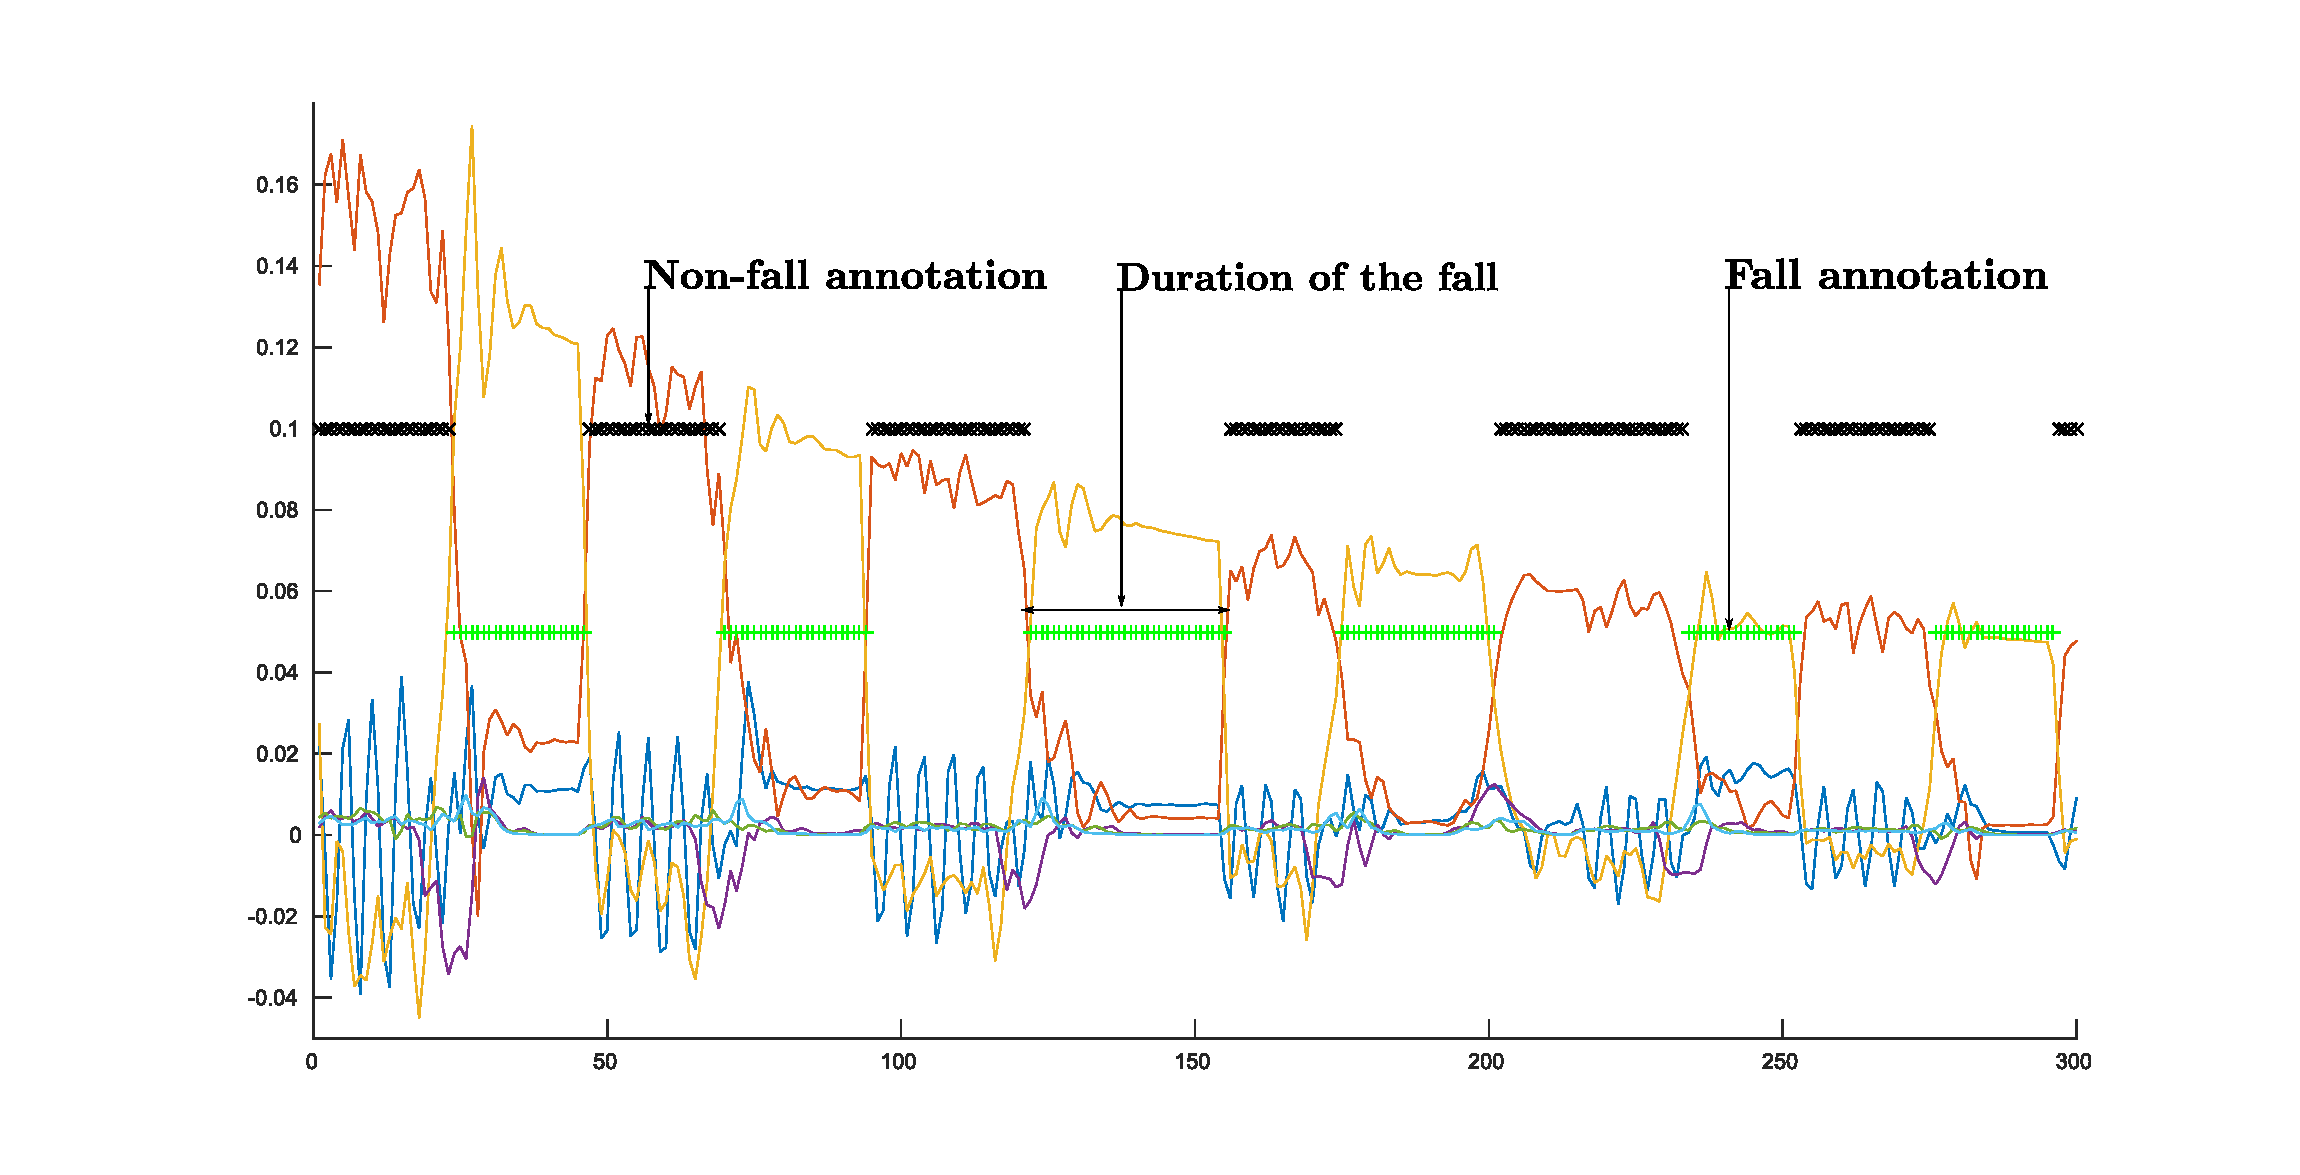
\includegraphics[width=0.45\textwidth]{plots/human_falling_forward2.eps} 
\caption{Semi-automatic annotation of falling forward event dataset.}
 \label{fig:automatic_annotation} 
\end{figure}


\begin{figure}[!tb]
\centering
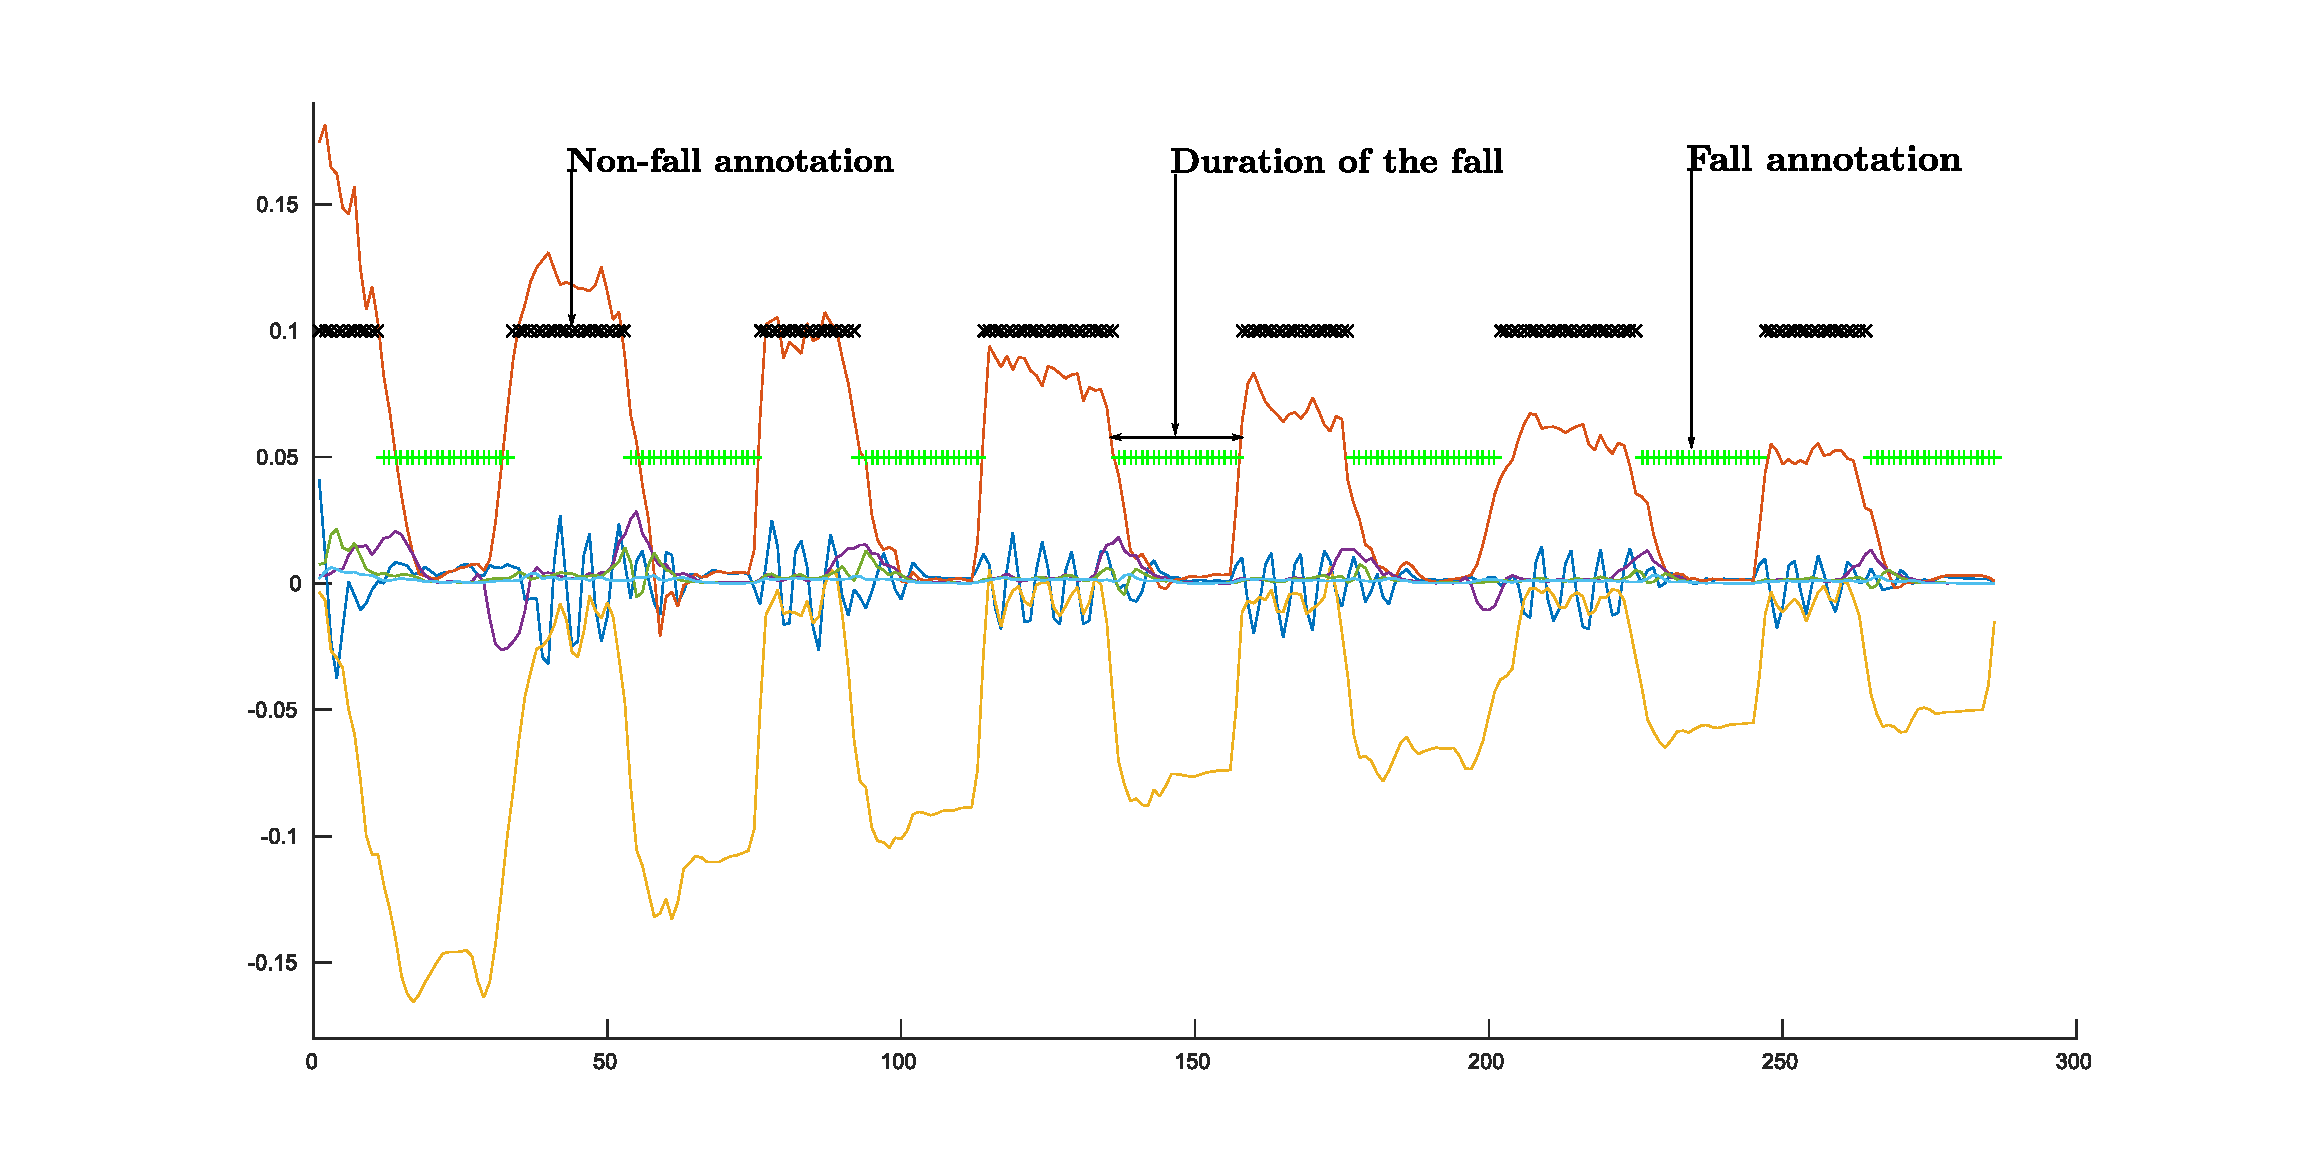
\includegraphics[width=0.45\textwidth]{plots/human_falling_backward2.eps} 
\caption{Semi-automatic annotation of falling backward event dataset.}
 \label{fig:automatic_annotation2} 
\end{figure}





%\begin{figure}[!t]
%\centering
%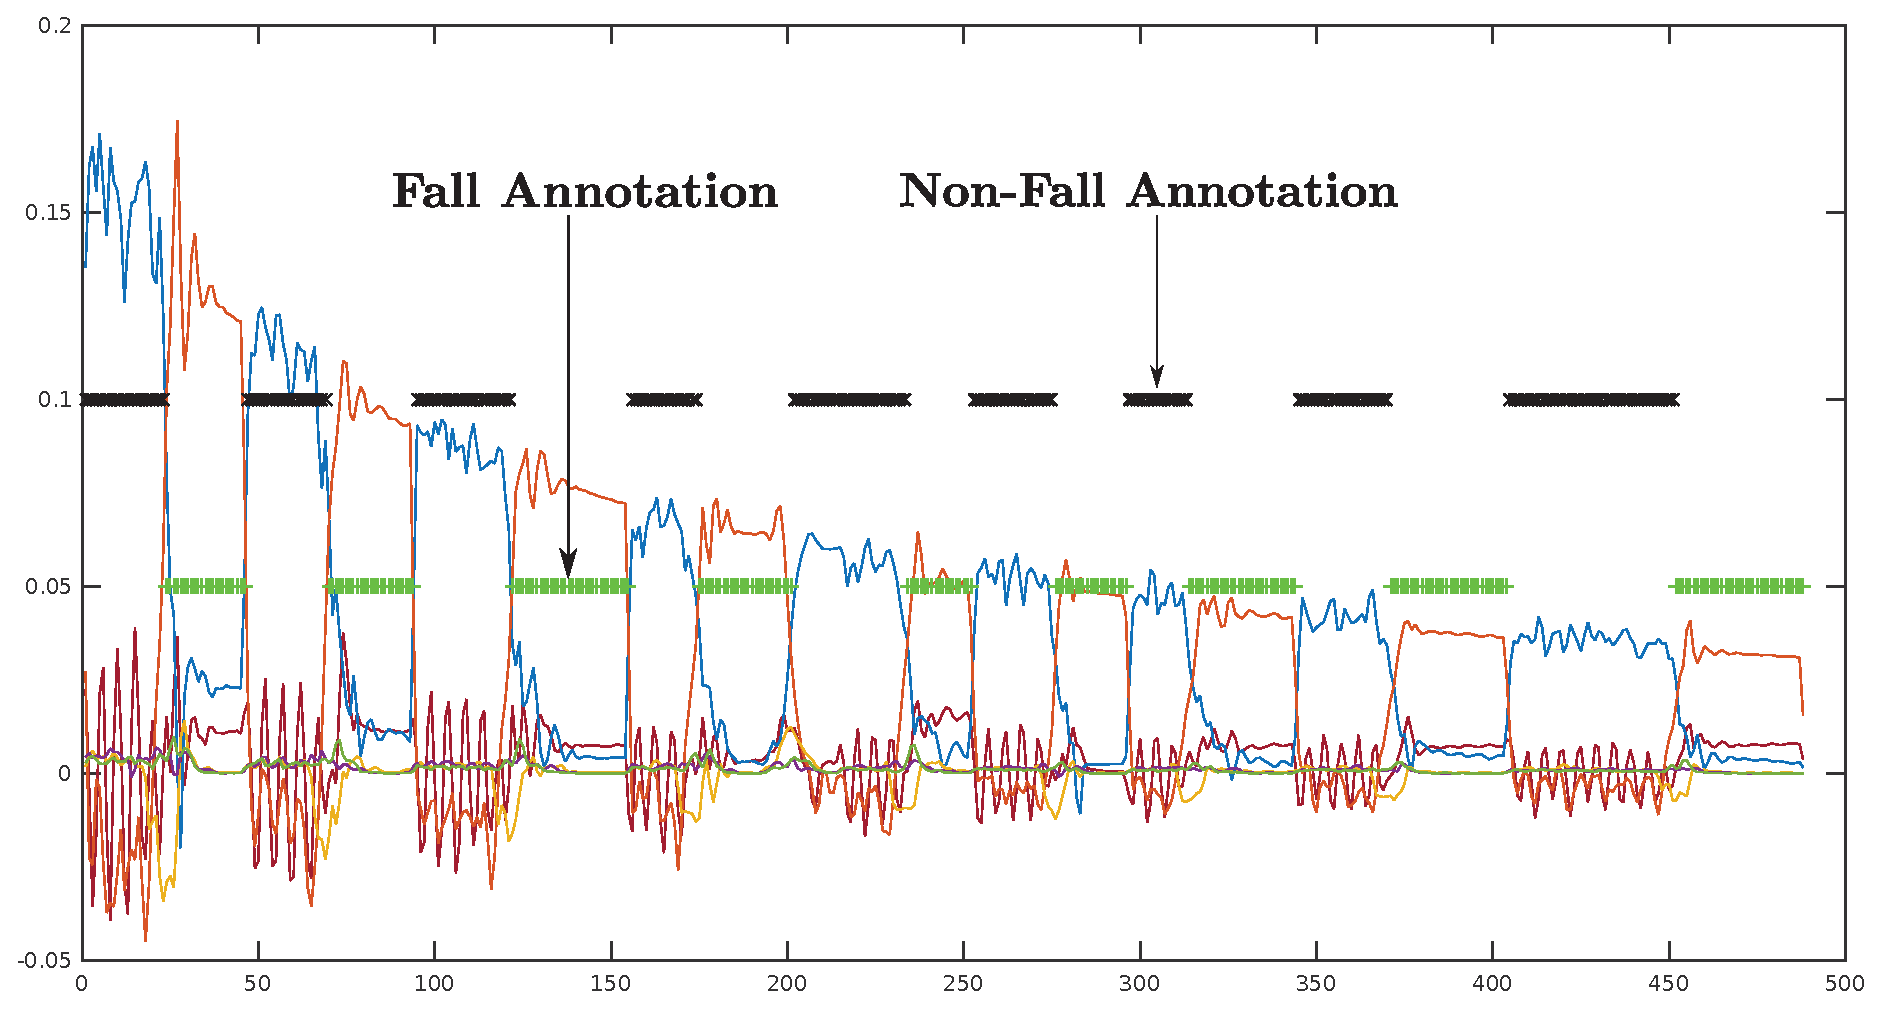
\includegraphics[width=0.48\textwidth]{figures/example_annotation-crop.eps} 
%\caption{Semi-automatic annotation of falling forward dataset.}
 %\label{fig:automatic_annotation} 
%\end{figure}


Figures~\ref{fig:automatic_annotation} and \ref{fig:automatic_annotation2} show plots and annotations of our semi-automatic annotation of falling-forward  and falling-backward datasets, respectively. The subject in this experiment simulated a fall froward. After a 
fall, the subject immediately gets up and repeats the process. The green ``+'' segments 
show the annotated fall events, while the black ``x'' segments show the non-fall 
events. We have observed that there is a clear separation of the events with two 
clusters. Each segment has between 15 to 20 consecutive data points.
% which amounts to 3000$ms$ to 4000$ms$ fall event after triggering the event. 
Each fall-event triggers 
towards the end of the preceding non-fall data points and continues into the beginning of the fall data points; this is the transition zone of a fall event.

\par
For visualization of 11 sets of training examples, a sample Tsne projection  is displayed in Fig.~\ref{fig:automatic_annotation3}. In this projection, the 4 fall events (numbered 1 through 4) show a clear separation from each other and all 7 non-fall events. Although, separation of non-fall events in Fig.~\ref{fig:automatic_annotation3} do not show as good separations, but our results show that they are far enough from each other for 100\% accurate classifications.

\begin{figure*}[!htb]
\centering
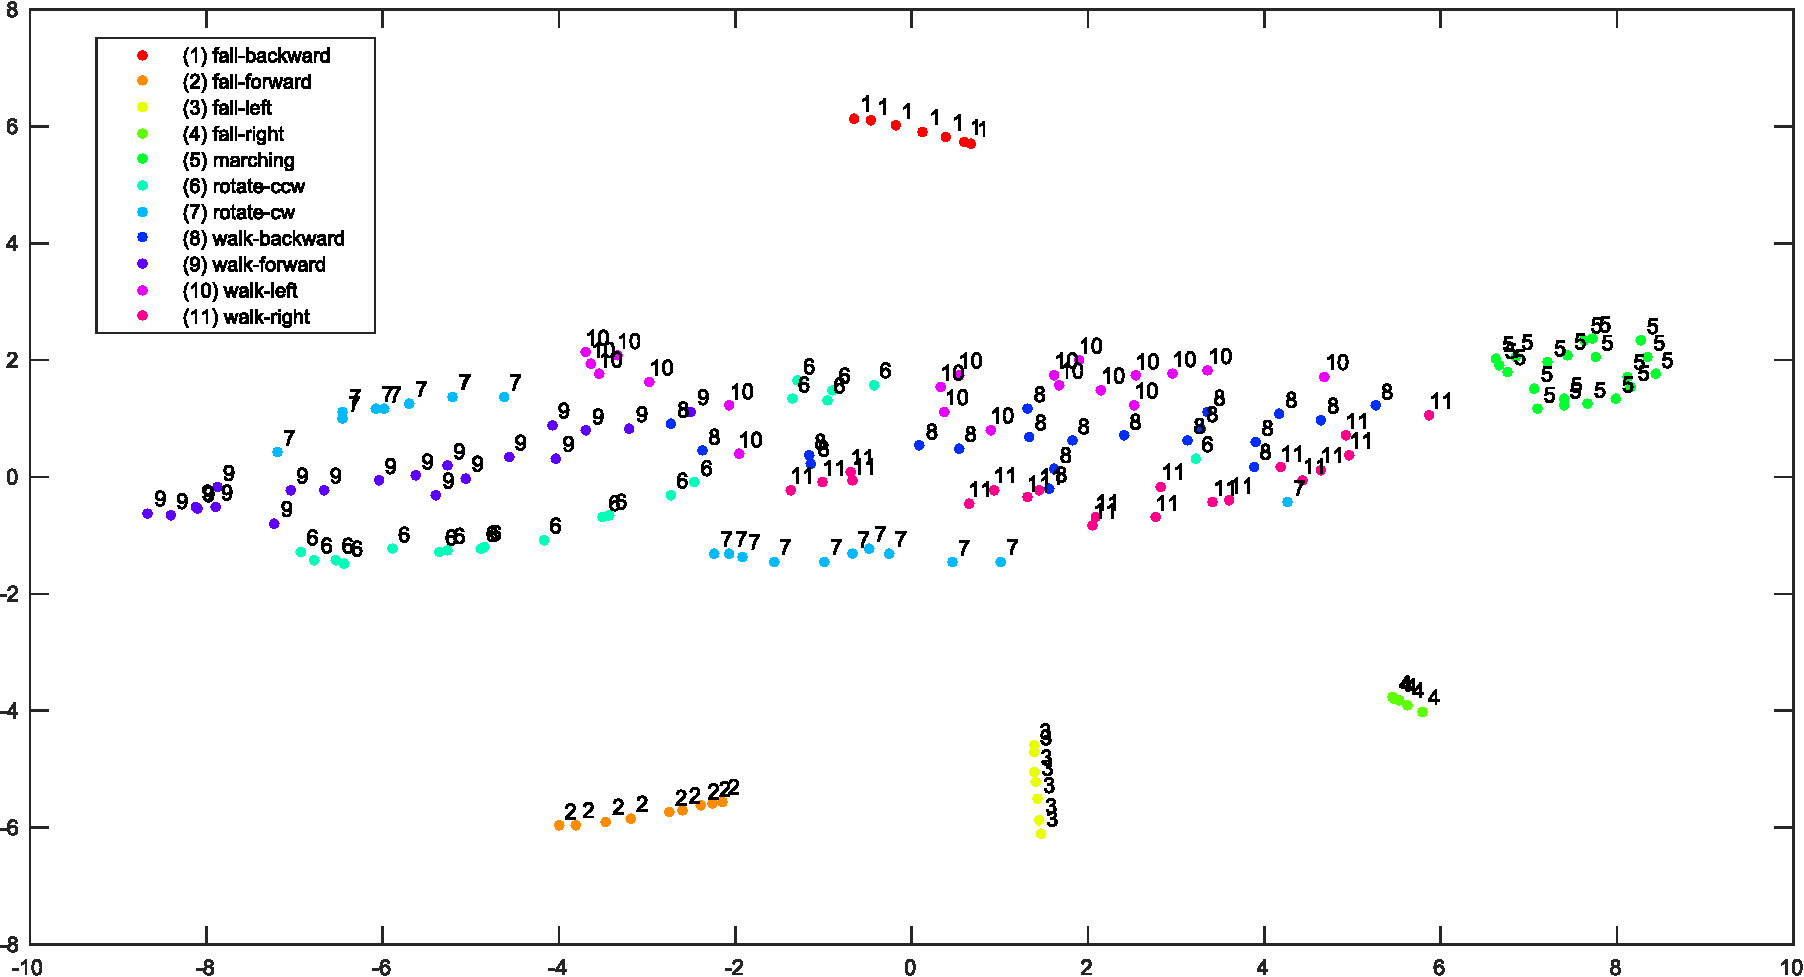
\includegraphics[width=.85\textwidth]{figures/viz_all_training_examples_crop2.pdf} 
\caption{Visualization of 11 sets of training examples using Tsne projection. In this projection, the 4 fall events (numbered 1 through 4) show a clear separation from each other and other 7 non-fall events.}
 \label{fig:automatic_annotation3} 
\end{figure*}


Since we are 
interested in the signatures of the fall events, we have annotated all the samples belongs 
to ``a'' cluster as the fall data. In general, the k-means clustering finds a 
local minimum. Moreover, the cluster assignments may vary depending on the 
initialization. Therefore, after we have obtained the data belongs to two clusters, we 
only have to manually provide the semantics of the cluster centroid. 

\section{Offline Learning and Predicting Algorithms}
\label{sec:OffLineLearning}

%TODO: About the algorithms we have used (SoftMax, ANN, and SVM).
%Trained the models using offline models. This is offline learning figure. 

Our activity monitoring and identification requires to learn and to predict beliefs of 
multiple 
discrete hypothesis. This includes learning and predicting dichotomies such as falling 
forward and 
backward, falling events and non-falling events, different types of falling events, and 
so forth. 
Therefore, 
we have used multi-class classification networks to rationally answer the question we 
have posed. We learn the classifiers offline from the training example extracted 
according to the methods presented in Section 
\ref{sec:SemiAutomaticExtractionOfTrainingVectors}. This section explains the classifiers 
that we have considered in our experiments and their configurations. 

Using our semi-automated training example extraction method, we have created $m \in 
\mathbb{N}$ 
training examples 
\{($\mathbf{x}^{(i)}, \mathbf{y}^{(i)}$)\}$_{i=1}^m$ such that $\mathbf{x} \in 
\mathbb{R}^{n}$ 
and 
$\mathbf{y} \in 
\{0,1\}^k$, where  $k \in 
\mathbb{N}$ is the number of dichotomies. Each training example belongs only to one class 
and $\mathbf{y}$ uses the 1--of--$k$ coding scheme.    

\subsection{Softmax Regression Algorithm}
\label{sec:SoftmaxRegrationAlgorthm}

The first classification network is based on Softmax regression \cite{Bishop06a}. In this 
model, given an 
example $\mathbf{x}$, it will determine the probability, $\mathbb{P}(y | \mathbf{x})$, 
for 
each dichotomy $y=0,\ldots,k-1$. The input is appended with constant bias 
term, $x_0 = 1$, therefore, $\mathbf{x} \in \mathbb{R}^7$. The model uses a parameter 
matrix 
$\mathbf{W} 
\in \mathbb{R}^{7 \times k}$, and the output vector, $\mathbf{a} = \mathbf{Wx}$, is 
passed 
through 
the 
Softmax 
activation function $\mathbf{z(a)} = \frac{e^{\mathbf{a}}}{\mathbf{1}^\mathtt{T}
e^{\mathbf{a}}}$, which represents the probability mass function $\mathbb{P}(y | 
\mathbf{x})$. We have 
used the regularized cross-entropy cost function as our objective function, 

\begin{equation} 
l(\mathbf{x}) = -\mathbf{y}.\ln \mathbf{z} + \frac{\lambda}{2} \mathbf{W}.\mathbf{W}
\label{eq:objective-function}
\end{equation}
 where  $\lambda$ is the regularization parameter, and ``.'' represents the scalar dot  
or Frobenius product.
 We have used L-BFGS \cite{DBLP:conf/icml/LeNCLPN11} to learn the 
parameter vector $\mathbf{W}$.  

\begin{figure}[htbp]
	\centering
		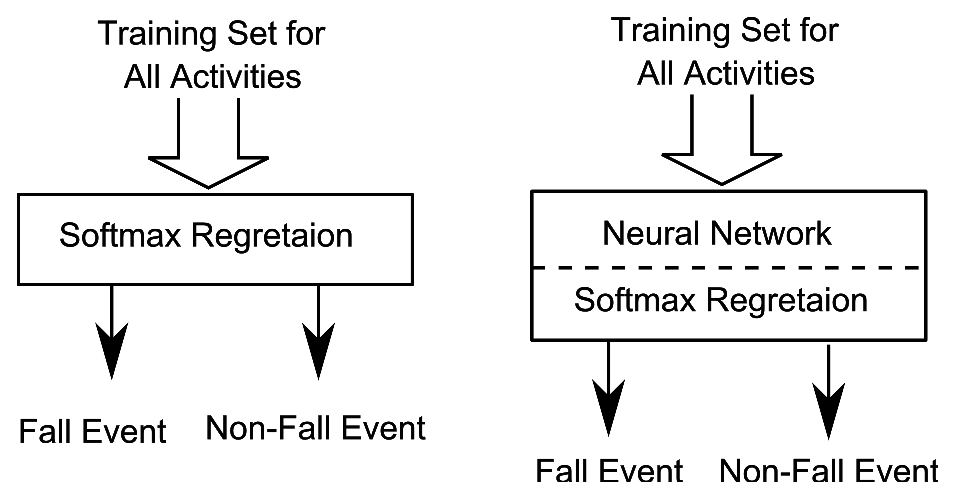
\includegraphics[width=0.75\columnwidth]{figures/SoftmaxLayer1.eps}
	\caption{Layer 1 learning modules. Examples are classified into Fall and Non-Fall events.  The left-side Figure is using Softmax Regression model. The Right-side Figure is a hybrid of Neural Network and Softmax Regression model.}
	\label{fig:SoftmaxLayer1}
\end{figure}

We trained and tested two networks with the Softmax regression algorithm. In the first case, we trained a one-layer network with 11 binary outputs, one for each fall or non-fall events. In the second case, we trained a two layer softmax regression network. The top layer network was trained with 2 binary outputs to distinguish between fall and non-fall events (see Fig.~\ref{fig:SoftmaxLayer1}). The bottom layer has two sub-networks:  one to identify fall events and has 4 binary outputs, the other to identify non-fall events and has 7 binary outputs. Each sub-network was trained separately. Fig.~\ref{fig:SoftmaxLayer2Fall} shows a block diagram of a subnetwork for training and identification of four fall events. For conserving space, we omit the diagram for non-fall events. As will be discussed in the next section, none of them identified all events with 100\% accuracy.

\begin{figure}[htbp]
	\centering
		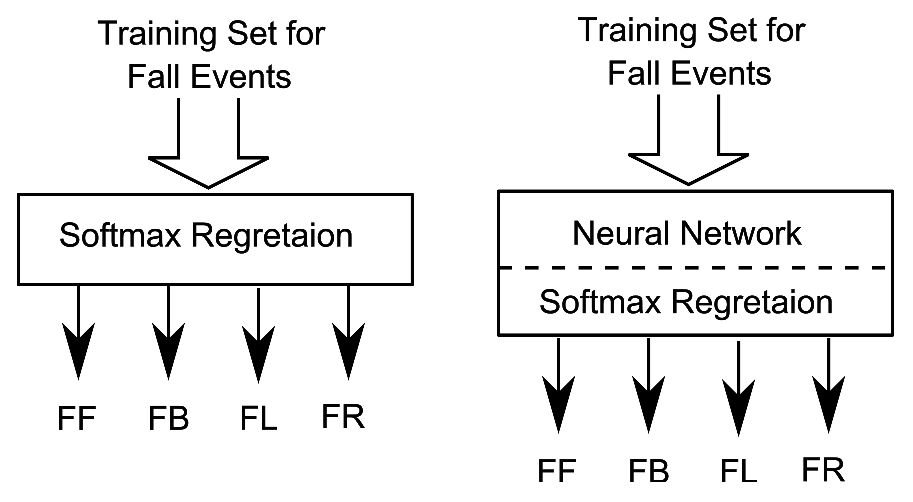
\includegraphics[width=0.75\columnwidth]{figures/SoftmaxLayer2Fall.eps}
	\caption{Layer 2 learning module for four Fall events. The left-side Figure is using Softmax Regression model. The right-side Figure is a hybrid of Neural Network and Softmax Regression }
	\label{fig:SoftmaxLayer2Fall}
\end{figure}

%\subsection{Neural Network}
%\label{sec:NeuralNetwork1}
%The second classification network is based on Artificial Neural Network \cite{Bishop06a}. 
%The network has configured with the same classification objective function as in the 
%previous section. We have 
%used the \emph{rectified linear unit  activation} (ReLU) in the hidden layers 
%\cite{AISTATS2011_GlorotBB11}. We have experimented with both one and two layer networks. 
%Performance of these networks are reported in the next section. None of them identified 
%all events with 100\% accuracy.

\subsection{Hybrid Algorithm: Neural Network with Softmax Regression}
\label{sec:HybridAlgorithmNeuralNetworkAndSoftmaxRegreation}

The hybrid classification network is based on both Artificial Neural Network  and Softmax regression network. Fig.~\ref{fig:SoftmaxLayer1} shows a block diagram of a hybrid network: a row of neurons followed by a row of softmax regression units.
\par
We have used the prior Softmax activation  and the negative-log likelihood 
functions in the output layer. The hidden layers have used \emph{rectified linear units }(ReLUs). 
We have also included the bias terms for all hidden layers. The backpropagation algorithm\cite{Sarkar1995}
has been used to calculate the gradient, while the L-BFGS procedure has been used to 
learn the network parameters. We have independently set each dimension of the sample to 
have zero-mean and unit-variance. We achieved this by first computing the mean of each 
dimension across the training set and subtracting this from each dimension. Then each 
dimension is divided by its standard deviation.       

Similar to Softmax regression networks, we experimented  with both single-layer hybrid networks and two-layer hybrid networks. While single-layer network failed to identify all events with 100\% accuracy, the two-layer network successfully identified all event with 100\% accuracy. There were no false positives or false negatives. In the rest of paper, we use hybrid networks and neural networks interchangeably.

\section{Online Activity Monitoring and Identification}

In Sections \ref{sec:SemiAutomaticExtractionOfTrainingVectors} and 
\ref{sec:OffLineLearning}, we have discussed the semi-automatic training example 
extraction and the learning of the parameter vectors of the classifiers for the event 
prediction and identification. This process is primarily offline. In operational mode, we 
require that the learned classifiers monitor and identify events online. This section 
provides our setup and methodology.  



\subsection{Monitoring of Events}

For the monitoring of events, we have followed a methodology similar to that of 
Subsection \ref{subsec:preDataCollection}. We have continuously collected the sample data 
to a circular buffer. From a starting marker (initially at the beginning of the circular buffer), 
we have averaged 20 consecutive sample and added that value to a second circular buffer. The 
first circular buffer is incremented by 10 samples, then average the next 20 samples (if the 
data 
is available), and pushed  the average value into the second circular buffer. We have 
continued this process in 
the first circular buffer with 10 samples overlap. In the second circular buffer, we have 
maintained a window of 20 samples. 
In order to compensate for noise, we have used five average values from the window. We 
have 
used the first 20, 18, 16, 14, and 12 average values. These  values are used in the event 
identification. We then incremented the second circular buffer by 10 samples and continued 
the process.  

\begin{figure}[h]
	\centering
		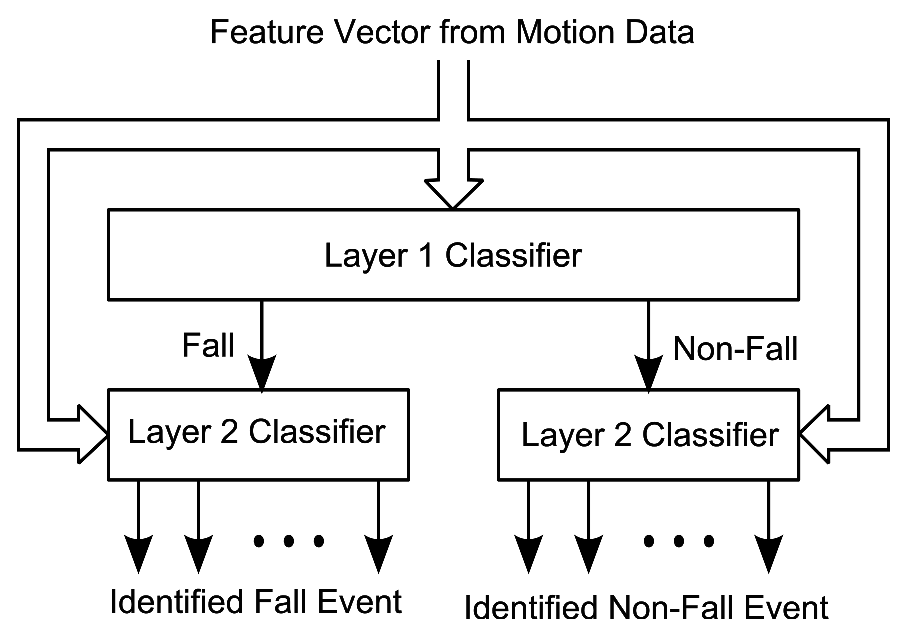
\includegraphics[width=0.365\textwidth]{figures/TrainedIdentificationModule.eps}
	\caption{Block diagram of event identification system. The top layer separates fall events from non-fall events. The bottom layer modules receive the same input data vector as the top layer, but they also get a zero or one input from the upper layer module depending on where the input data vector is classified. The final output is a binary valued vector of 11 components.}
	\label{fig:TrainedIdentificationModule}
\end{figure}


\subsection{Identification of Events}

As stated earlier and discussed in Section~\ref{Evaluation} for 100\% success rate, we have used a layered classification network as 
shown in Fig. \ref{fig:TrainedIdentificationModule}. The inputs to the classifiers are 
the 
pre-processed motion data from the previous subsection. In the first layer of our 
classification network (Layer 1), we have used a binary decision classifier that predicts 
whether the current input is a fall or a non-fall. Based on this decision, at the second 
layer of our network (Layer 2), one of the specific fall event or non-fall activity 
recognition classification network is activated. The decision of this classifier is 
considered as the output of the classification network. In order to compensate for noise, 
we have used the five samples as described in the previous section. We have marked the 
predicted events; if the five inputs (calculated from a window of the second circular 
buffer) 
predict the same outcome, then the network voted 
to that event, otherwise, we have identified an inconclusive event. 



\section{Empirical Evaluation of Proposed Algorithms and Methods}
\label{Evaluation}

In this section we report the performance of our proposed algorithms and methods. A detailed description of the data collection and preprocessing steps can be found in Section \ref{subsec:preDataCollection}.
%First we brieflydescribe our data collection procedure. 
We have experimented with one-layer and two-layer classifiers.  First, the performance of one-layer softmax and neural networks classifiers are reported. Then that for two-layer networks are presented. 
\emph{For all results reported here the value of $\lambda$ in the cost function 
(Equation~\ref{eq:objective-function}) is $0.1$.}

%\subsection{Data Collection}
%\label{Sec:dataCollection}
\begin{table}[htb]
\caption{Performance of a single layer Softmax regression network with six inputs and 11 outputs. On an average 94.4\% of the events were classified correctly.}
\label{tab:softmaxOnelayer}
\resizebox{\columnwidth}{!}
{
\begin{tabular}{|c|c|c|c|c|c|c|c|c|c|c|c|}
\hline 
& \textbf{FF} & \textbf{FB}  & \textbf{FL} & \textbf{FR} &  \textbf{WF} & 
\textbf{WB} & \textbf{WL} & \textbf{WR} & \textbf{MR} & 
\textbf{RC} & \textbf{RA} \\ \hline
\textbf{FF} & 66.7 &  0 &  0 &  0 &  0 &  16.7 &  0 &  0 &  16.7 &  0 &  0 \\ \hline
\textbf{FB} & 0 &  100 &  0 &  0 &  0 &  0 &  0 &  0 &  0 &  0 &  0 \\ \hline
\textbf{FL} & 0 &  0 &  100 &  0 &  0 &  0 &  0 &  0 &  0 &  0 &  0 \\ \hline
\textbf{FR} & 0 &  0 &  0 &  100 &  0 &  0 &  0 &  0 &  0 &  0 &  0 \\ \hline
\textbf{WF} & 0 &  0 &  0 &  0 &  87.5 &  0 &  0 &  12.5 &  0 &  0 &  0 \\ \hline
\textbf{WB} & 0 &  0 &  0 &  0 &  0 &  100 &  0 &  0 &  0 &  0 &  0 \\ \hline
\textbf{WL} & 0 &  0 &  0 &  0 &  0 &  0 &  100 &  0 &  0 &  0 &  0 \\ \hline
\textbf{WR} & 0 &  0 &  0 &  0 &  0 &  0 &  12.5 &  87.5 &  0 &  0 &  0 \\ \hline
\textbf{MR} & 0 &  0 &  0 &  0 &  0 &  0 &  0 &  0 &  100 &  0 &  0 \\ \hline
\textbf{RC} & 0 &  0 &  0 &  0 &  0 &  0 &  0 &  0 &  0 &  100 &  0 \\ \hline
\textbf{RA} & 0 &  0 &  0 &  0 &  0 &  0 &  0 &  0 &  0 &  0 &  100 \\ \hline
\end{tabular}
}
\end{table}
%We have conducted our experiments on detecting seven non-fall movement activities and four fall events on 
%%able-bodied 
%humans. The list of these activities and fall events with their abbreviations are shown in
%Table~\ref{Tbl:ListOfActivities}. 
%
 %As shown in Fig.~\ref{fig:deviceWithSubjects}, a wireless 9-axis  motion sensing device was attached to the back of the subjects and a wireless data collecting device was connected to a computer. These two devices formed a wireless sensor network.
%\par
 %While a subject performed prescribed activities and simulated-fall events, data was logged in a computer. The collected datasets are  used
%for extracting training examples for learning algorithms as well as  performance evaluation purpose.
%The motion data included 3-axis accelerometer readings, 3-axis gyroscope readings, and 3-axis magnetometer readings. For results reported in this paper we did not use magnetometer readings. Figures \ref{fig:human_fall_forward_crop} and \ref{fig:human_walk_forward-crop} show plots of motion data for\begin{inparaenum}[($i$)] \item fall forward and \item walk forward\end{inparaenum}, respectively.
 %



\subsection{One-Layer Networks}
\label{sec:SingleLayerNetworks}
We  trained two one-layer networks: softmax regression and neural networks (see Fig.~\ref{fig:SoftmaxLayer1} for block diagrams of these networks). Performance of these networks are discussed in the next two paragraphs.
 
 \paragraph{Softmax Regression}
 \label{sec:SoftmaxRegression}
 As can be seen from Table~\ref{tab:softmaxOnelayer}, one-layer sofmax regression network with 7 inputs (6 for feature vector and one for bias) and 11 outputs recognized on an average 94.4\% of all  events. A closer examination reveals that all but three types of events --- fall-forward, walk-forward, and walk-right events  --- are recognized correctly. Recognition rate for fall-forward events is only 66.7\%. This event is sometimes  incorrectly classified as a 
walk backward or a march event. Walk forward event is correctly recognized on an average rate of 87.5\% and sometimes it is incorrectly classified as a walk-right event. Recognition rate for walk right events is same as walk forward and is confused with  some  walk-left events.
\begin{table}[htb]
\caption{Performance of a Neural network with one row of neurons with ReLU and one row of elements with softmax activation function. On an average 95.8\% of the events were classified correctly.}
\label{tbl:neuralNetworkOneLayer}
\resizebox{\columnwidth}{!}
{
\begin{tabular}{|c|c|c|c|c|c|c|c|c|c|c|c|}
\hline 
& \textbf{FF} & \textbf{FB}  & \textbf{FL} & \textbf{FR} &  \textbf{WF} & 
\textbf{WB} & \textbf{WL} & \textbf{WR} & \textbf{MR} & 
\textbf{RC} & \textbf{RA} \\ \hline
\textbf{FF} & 66.7 &  0 &  0 &  0 &  0 &  0 &  16.7 &  0 &  16.7 &  0 &  0 \\ \hline
\textbf{FB} & 0 &  100 &  0 &  0 &  0 &  0 &  0 &  0 &  0 &  0 &  0 \\ \hline
\textbf{FL} & 0 &  0 &  100 &  0 &  0 &  0 &  0 &  0 &  0 &  0 &  0 \\ \hline
\textbf{FR} & 0 &  0 &  0 &  100 &  0 &  0 &  0 &  0 &  0 &  0 &  0 \\ \hline
\textbf{WF} & 0 &  0 &  0 &  0 &  100 &  0 &  0 &  0 &  0 &  0 &  0 \\ \hline
\textbf{WB} & 0 &  0 &  0 &  0 &  0 &  100 &  0 &  0 &  0 &  0 &  0 \\ \hline
\textbf{WL} & 0 &  0 &  0 &  0 &  0 &  0 &  100 &  0 &  0 &  0 &  0 \\ \hline
\textbf{WR} & 0 &  0 &  0 &  0 &  0 &  0 &  12.5 &  87.5 &  0 &  0 &  0 \\ \hline
\textbf{MR} & 0 &  0 &  0 &  0 &  0 &  0 &  0 &  0 &  100 &  0 &  0 \\ \hline
\textbf{RC} & 0 &  0 &  0 &  0 &  0 &  0 &  0 &  0 &  0 &  100 &  0 \\ \hline
\textbf{RA} & 0 &  0 &  0 &  0 &  0 &  0 &  0 &  0 &  0 &  0 &  100 \\ \hline
\end{tabular}
}
\end{table}

\paragraph{Neural Network}
\label{sec:NeuralNetwork2}
Performance of neural networks is shown in Table~\ref{tbl:neuralNetworkOneLayer}; it recognized 95.8\% of all events correctly. Before we discuss our results, it should be noted that the network is composed of one hidden row of  16 neurons with ReLU followed by a row of 11 elements with softmax activation function (see Fig.~\ref{fig:SoftmaxLayer1} in Section~\ref{sec:OffLineLearning}). An advantage of this architecture is that the number of neurons in the hidden row  can be varied for optimal performance.

\par
As can be seen from Table~\ref{tbl:neuralNetworkOneLayer}, all events except fall-forward and walk-right events were recognized correctly. The neural network improved recognition rate of walk-forward events to 100\%. But recognition rates of 
fall-forward and walk-right events remained same as softmax network at 66.7\% and 87.5\%, respectively.
\par
Because of failure of one-layer networks, we explored two-layer classification networks: the first layer classified an input into two categories, a fall event or a non-fall event. Then, a second layer  differentiated events within its own category. A block diagram of the classifier  is shown in Fig.~\ref{fig:TrainedIdentificationModule}.
\subsection{Two-Layer Networks}
\label{sec:TwoLayerNetworks}
\begin{table}[htb]
\caption{ Performance of layer-one of a two-layer classifiers. Softmax network at layer-one correctly identified 87.17\% of fall events from non-fall events, but the neural network correctly identified all fall and non-fall events.}
\label{tbl:layer1RecognitionRates}
\resizebox{\columnwidth}{!}
{
\begin{tabular}{|c|c|c||c|c|}
\hline
& \multicolumn{2}{c||}{\bf Softmax L1: 87.2} & \multicolumn{2}{c|}{\bf Neural L1: 
100} \\ \hline
& \textbf{Fall Event} & \textbf{Non-Fall Event}  & \textbf{Fall Event} & \textbf{Non-Fall 
Event} \\ \hline
\textbf{Fall Event} & 85.7 &  14.3  & 100 &  0 \\ \hline
\textbf{Non-Fall Event} & 12.7 &  87.3 & 0 &  100 \\ \hline
\end{tabular}
}
\end{table}

\subsubsection{Layer One - Classification of Fall Events or Non-fall Activities }
\label{sec:LayerOneFallAndNonFallIdentification}

Performance of layer-one of a two-layer classifiers has been tabulated in Table~\ref{tbl:layer1RecognitionRates}. As can be seen from the table, softmax network at layer-one (top layer) correctly classified only 87.2\% of fall and non-fall events, but neural network correctly classified all fall and non-fall events. We used only two neurons in the hidden row.
\par
 Because of its 100\% recognition rate we choose neural networks as layer-one network. In the subsequent discussion, unless otherwise mentioned,  layer-one classifier is a neural network with two hidden units.

%\paragraph{Siftmax Regression}
%\label{sec:SiftmaxRegression}
%
%\paragraph{Neural Network}
%\label{sec:NeuralNetwork}

\subsubsection{Layer Two - Identification of Individual Fall Events or Non-fall 
Activities}
\label{sec:LayerTwoFallOrNonFallEventIdentification}

the performances of layer-two networks are shown in Tables~\ref{Layer2FallEvents}, \ref{Layer2NonFallEventsSoftmax}, and \ref{Layer2NonFallEventsNeuralNets}. It is easy to see from Table~\ref{Layer2FallEvents} that both Softmax and Neural networks at layer-two correctly classified 100\% of fall events.
Results for seven non-fall events are shown in Tables~\ref{Layer2NonFallEventsSoftmax} and 
\ref{Layer2NonFallEventsNeuralNets}. Again both Softmax and Neural networks achieved 100\% accuracy. The neural network used one hidden row of 6 neurons.
\begin{table}[htb]
\resizebox{\columnwidth}{!}
{
\begin{tabular}{|c|c|c|c|c||c|c|c|c|}
\hline 
& \multicolumn{4}{c||}{\bf Softmax: L2 Fall Event: 100} & \multicolumn{4}{c|}{\bf Neural 
L2 Fall Event: 100} \\ \hline
& \textbf{FF} & \textbf{FB}  & \textbf{FL} & \textbf{FR} & \textbf{FF} & \textbf{FB}  & 
\textbf{FL} & \textbf{FR} \\ \hline
\textbf{FF} & 100 &  0 &  0 &  0  & 100 &  0 &  0 &  0\\ \hline
\textbf{FB} & 0 &  100 &  0 &  0  & 0 &  100 &  0 &  0\\ \hline
\textbf{FL} & 0 &  0 &  100 &  0  & 0 &  0 &  100 &  0\\ \hline
\textbf{FR} & 0 &  0 &  0 &  100  & 0 &  0 &  0 &  100 \\ \hline
\end{tabular}
}
\caption{ Performance of layer-2 network for  four fall events. Both softmax and neural networks correctly classified 100\% of fall events.}
\label{Layer2FallEvents}
\end{table}



\begin{table}[htb]
\caption{Performance of layer-2 network for  seven non-fall events. Softmax networks correctly classified 100\% of non-fall events.}
\label{Layer2NonFallEventsSoftmax}
%\resizebox{\columnwidth}{!}
\centering
{
\begin{tabular}{|c|c|c|c|c|c|c|c|}
\hline 
 & \textbf{WF} & \textbf{WB} & \textbf{WL} & \textbf{WR} & \textbf{MR} & 
\textbf{RC} & \textbf{RA} \\ \hline    
\textbf{WF} & 100 &  0 &  0 &  0 &  0 &  0 &  0 \\ \hline
\textbf{WB} & 0 &  100 &  0 &  0 &  0 &  0 &  0 \\ \hline
\textbf{WL} & 0 &  0 &  100 &  0 &  0 &  0 &  0 \\ \hline
\textbf{WR} & 0 &  0 &  0 &  100 &  0 &  0 &  0 \\ \hline
\textbf{MR} & 0 &  0 &  0 &  0 &  100 &  0 &  0 \\ \hline
\textbf{RC} & 0 &  0 &  0 &  0 &  0 &  100 &  0 \\ \hline
\textbf{RA} & 0 &  0 &  0 &  0 &  0 &  0 &  100 \\ \hline
\end{tabular}
}
\end{table}



\begin{table}[htb]
\caption{Performance of layer-2 network for  seven non-fall events. Neural networks correctly classified 100\% of  seven non-fall events.}
\label{Layer2NonFallEventsNeuralNets}
%\resizebox{\columnwidth}{!}
\centering
{
\begin{tabular}{|c|c|c|c|c|c|c|c|}
\hline 
 & \textbf{WF} & \textbf{WB} & \textbf{WL} & \textbf{WR} & \textbf{MR} & 
\textbf{RC} & \textbf{RA} \\ \hline 
\textbf{WF} & 100 &  0 &  0 &  0 &  0 &  0 &  0 \\ \hline
\textbf{WB} & 0 &  100 &  0 &  0 &  0 &  0 &  0 \\ \hline
\textbf{WL} & 0 &  0 &  100 &  0 &  0 &  0 &  0 \\ \hline
\textbf{WR} & 0 &  0 &  0 &  100 &  0 &  0 &  0 \\ \hline
\textbf{MR} & 0 &  0 &  0 &  0 &  100 &  0 &  0 \\ \hline
\textbf{RC} & 0 &  0 &  0 &  0 &  0 &  100 &  0 \\ \hline
\textbf{RA} & 0 &  0 &  0 &  0 &  0 &  0 &  100 \\ \hline
\end{tabular}
}
\end{table}



\section{Conclusions and Future Work}

%While humans perform activities of daily life, an accident 
%such as a fall may occur. This might cause injuries to the human body, and immediate identification of it can alert for a fast response.  
During activities of daily life, an accident 
such as a fall may occur to humans. This may lead to injuries, and immediate identification of it can alert for a fast response.  There are many inexpensive wireless motion sensing devices or one can be assembled using off-the-shelf components. These devices can be attached to a human to collect motion data for monitoring activities of daily living. However, while performing these activities, an accident such as fall may occur.

We have developed a generic software platform for embedded devices. The software platform has been tested on several combinations of microcontrollers and sensing devices. We have used it for creating a wireless sensor network and using the network for collecting motion data.

In order to accurately identify these events, it is necessary to extract distinguishing features from the motion data. Here, we have proposed a novel semi-automatic training example extraction method to identify features and automatically annotate the datasets. The proposed method significantly  expedites the creation of the training set compared to manually extracting them. Moreover, we have proposed and implemented a two-level classification network with  a combination of neural and softmax regression networks to identify seven type of non-fall activities and four types of fall events with 100\% accuracy. 

While the evaluation of the proposed techniques using our off-the-shelf device has proven to be effective, the project is far from complete. It requires further testing. Also, for real-world deployment, a miniaturized prototype must be developed and tested on a wide population. We expect that the software platform will require only minimum modifications, if at all.

\bibliographystyle{plain}
\bibliography{references,fallRisk}

%\end{sloppy}
\end{document}
